%!TEX TS-program = xelatex
%!TEX root = ../../maxwell2018thesis.tex

\chapter[General Methodology]{General Methodology}\label{chap:method}
In Part~\ref{part:context}, we will be exploring how an individual's stopping behaviours vary under different search contexts. In this chapter, we provide an overview of the general methodology that we deploy in subsequent chapters. As per the overview provided in Chapter~\ref{chap:intro}, our methodology is divided into four main areas:

\begin{itemize}
    \item{conducting a \blueboxbold{user study} to examine real-world searcher behaviours;}
    \item{extracting the key \blueboxbold{interaction data and performance measures} from the user study;}
    \item{using the aforementioned data to ground a series of \blueboxbold{simulations} that attempt to replicate the user studies; and}
    \item{\blueboxbold{evaluating} the performance of the simulated users, as well as \blueboxbold{comparing} the simulated user behaviours against those of their real-world counterparts.}
\end{itemize}

We now discuss each of these different tasks in greater depth, highlighting the key decisions that we have made, and discuss supporting literature for our choices.

\section{Test Collection, Topics and Search Engine}\label{sec:csm:methodology:collection}
Central to any~\gls{acr:ir} experiment is a corpus of documents (refer to Section~\ref{sec:ir_background:basics:indexing}) with which subjects participating in the experiment can issue queries against. In conjunction with the document corpus, a number of topics are also used to provide simulated information needs.

For the contributory chapters of this thesis, all work detailed uses the TREC AQUAINT corpus, consisting of over one million news articles (referred to as documents) from the period ranging 1996 to 2000. All of the news articles were collected from three newswires, namely: the \emph{Associated Press (AP);} the \emph{New York Times (NYT);} and \emph{Xinhua}. More contemporary collections could have been used; the reasons for selecting an older were twofold: \emph{(i)} using such a collection enabled us to easily evaluate the performance of subjects; and \emph{(ii)} employing the AQUAINT corpus provides continuity with a prior line of research using this collection, as shown by~\cite{azzopardi2013query_cost}, for example.

Five topics were also selected from the 50 provided in the \emph{TREC 2005 Robust Track,} as outlined by~\cite{voorhees2006trec_robust}. These topics were selected based upon evidence from a previous user study (of similar nature) conducted by~\cite{kelly2015serp_size}. Evidence showed that the topics offered similar levels of difficulty. The five topics, along with a short description of what constitutes a relevant document, are listed below. These summaries are derived from the TREC topic descriptions that are provided as part of the TREC 2005 Robust Track -- Figure~\ref{fig:topics} illustrates three examples of topic descriptions.

\begin{figure}[t!]
    \centering
    \resizebox{1\hsize}{!}{
    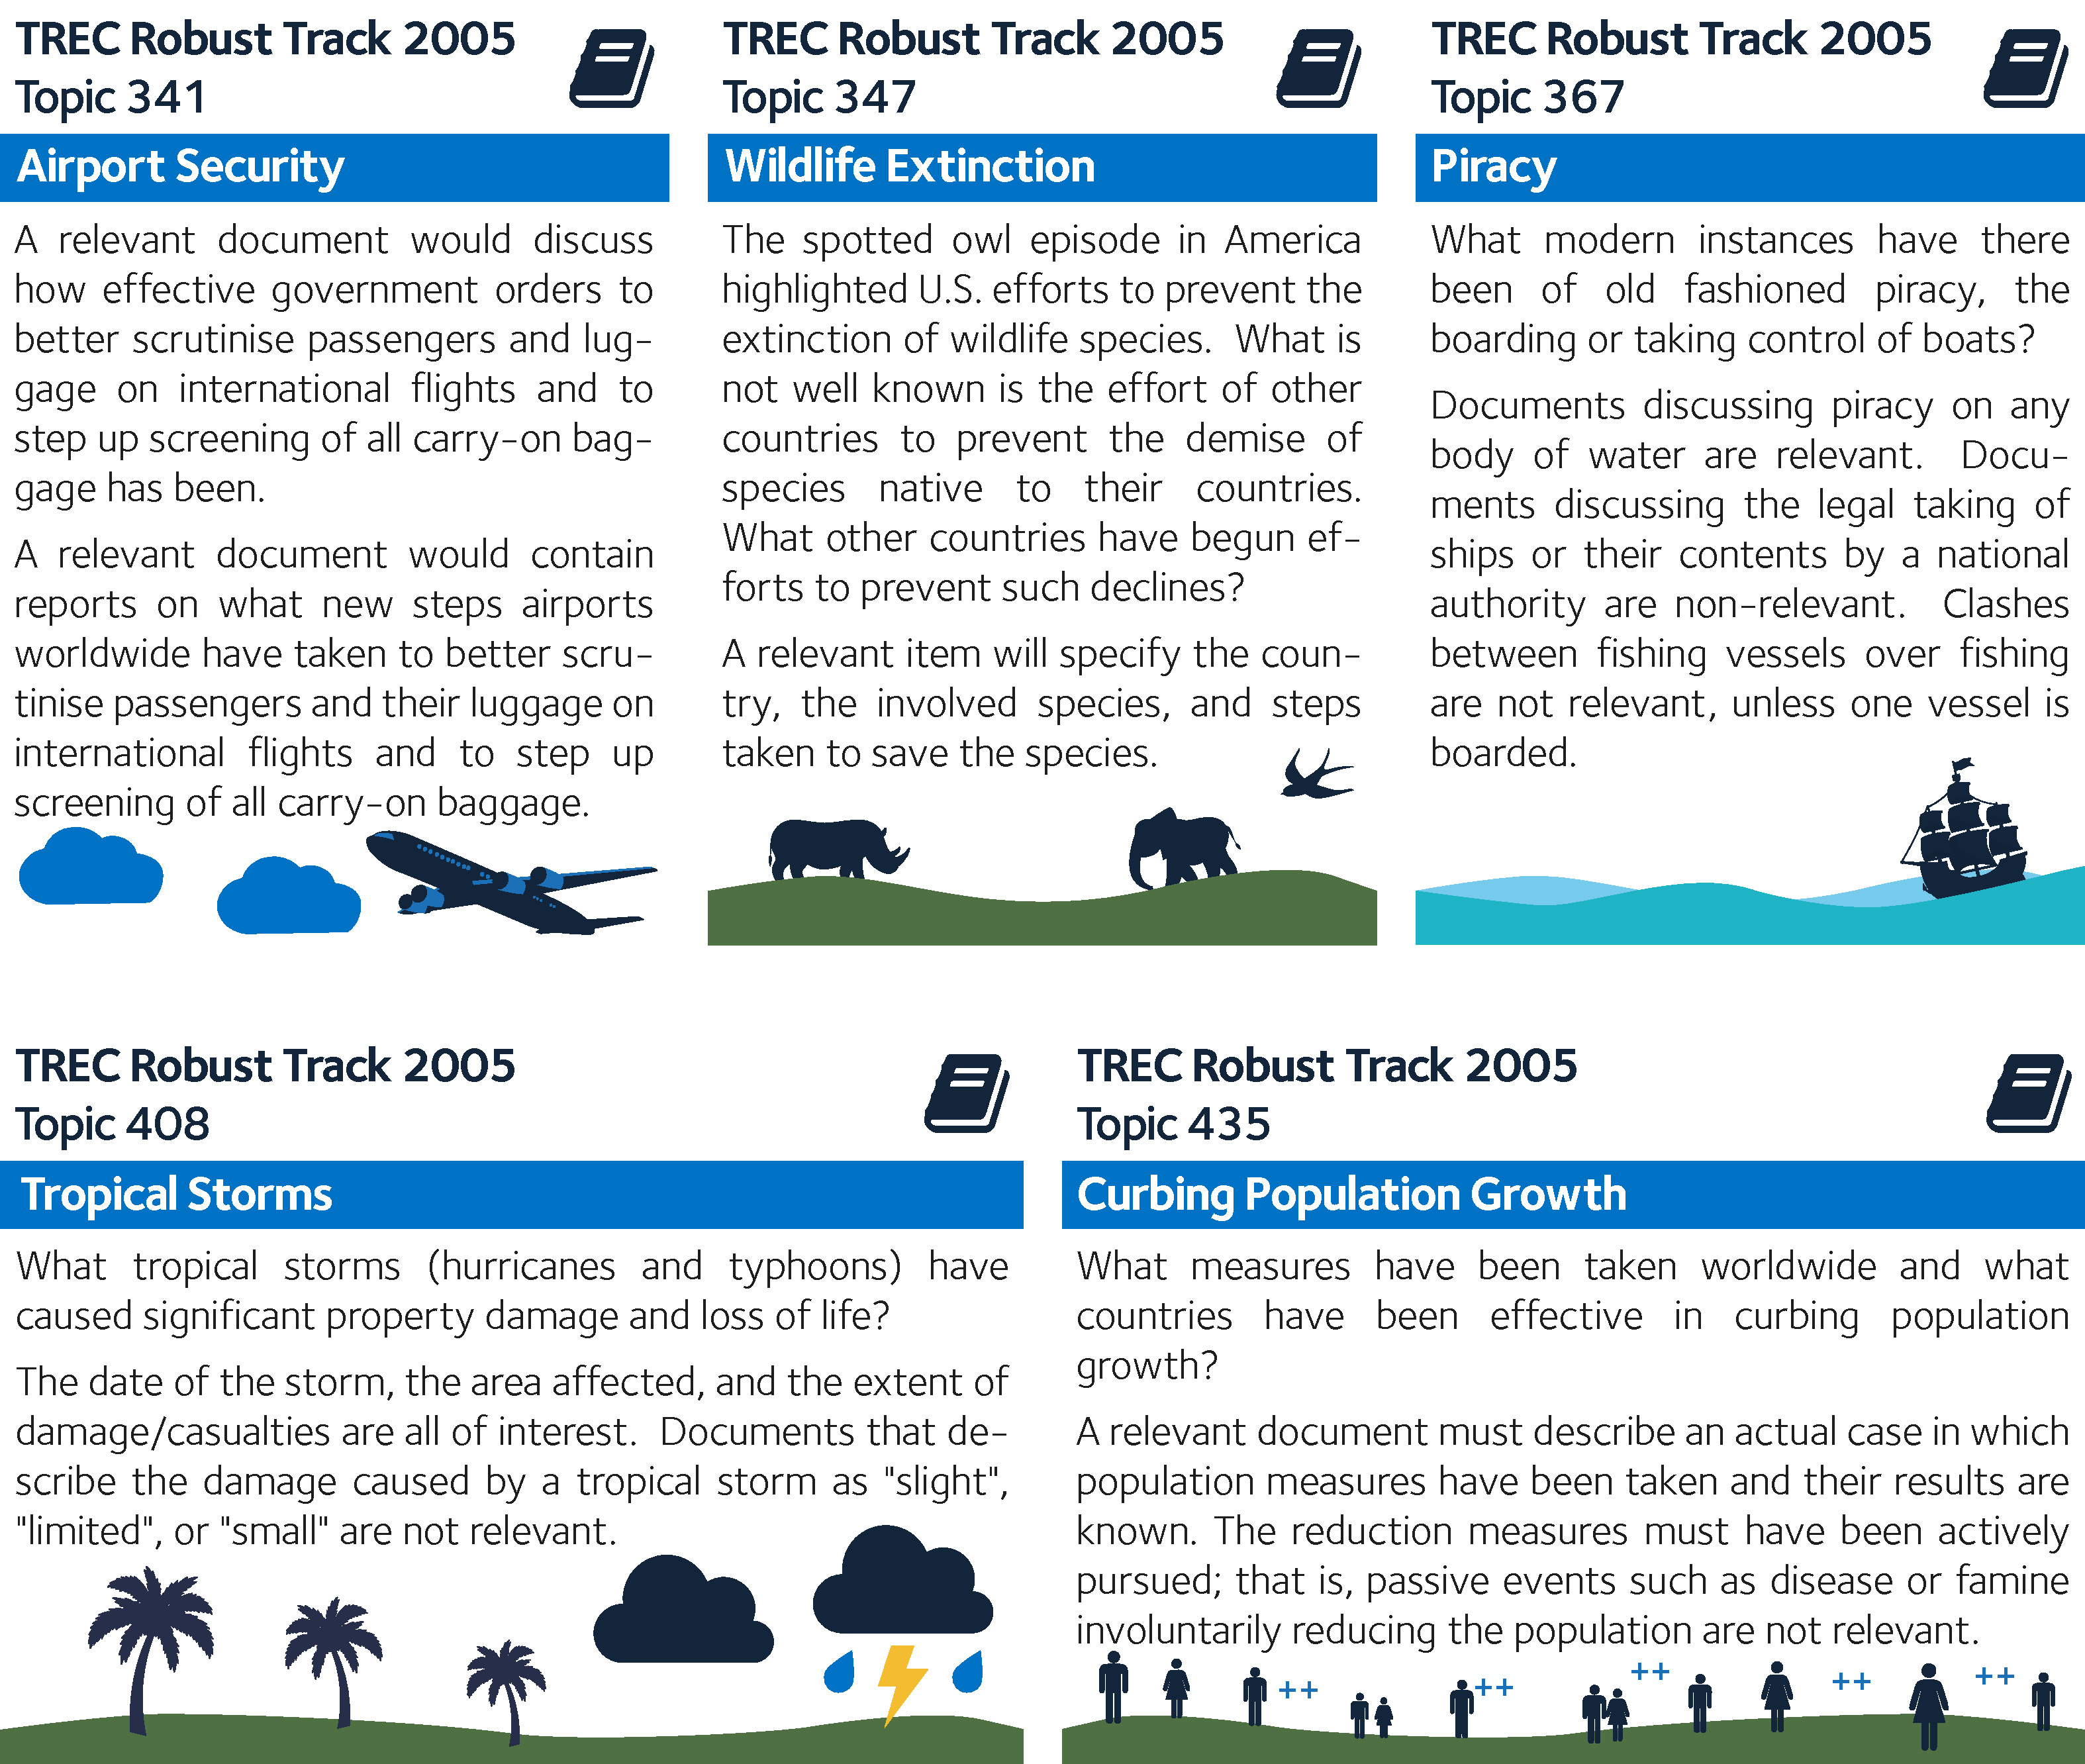
\includegraphics{figures/ch4-topics.pdf}}
    \caption[Examples of TREC Topics]{Three examples of \emph{TREC topic descriptions}, as outlined in Section~\ref{sec:csm:csm:flow}. Topics are extracted from the \emph{TREC 2005 Robust Track,} as outlined by~\cite{voorhees2006trec_robust}. Descriptions provide an explanation as to what constitutes a relevant (and often non-relevant) document.}
    \label{fig:topics}
\end{figure}

\begin{itemize}
    
    \item[]{\blueboxbold{Topic 341 – Airport Security} This topic considers relevant documents as those that discuss additional security measures that were taken by international airports around the world. Relevance is only denoted when a document discusses measures that go beyond the basic passenger and carry-on luggage screening. For example, AQUAINT document \texttt{NYT19980616.0123} discusses \emph{San Francisco International Airport's} attempts at introducing a \emph{robot sniffer,} attempting to look for nitroglycerine in luggage.}
    
    \item[]{\blueboxbold{Topic 347 – Wildlife Extinction} As the title of the topic suggests, this topic concerns wildlife extinction, and what efforts have been taken by countries other than the United States to counter the decline in endangered wildlife. Relevant documents explicitly mention the country, the species of animal, and the efforts the state or other governmental agency took to prevent decline in numbers. For example, document \texttt{XIE20000531.0205} discusses the breeding programme undertaken by China to bolster the number of Siberian Tigers in its jurisdiction.}
    
    \item[]{\blueboxbold{Topic 367 – Piracy} Instances of modern piracy are considered relevant to this topic -- not in the sense of software piracy, but the act of a water going vessel being boarded by individuals wishing to hijack it. Document \texttt{APW19980601.1065} provides an example of this -- the \emph{Petro Ranger}, a large fuel tanker, was boarded by pirates in 1998 in the South China Sea. To be relevant to the topic, the name of the vessel and the body of water it was hijacked on must be mentioned -- those discussing instances of when states intercepted vessels are not relevant.}
    
    \item[]{\blueboxbold{Topic 408 – Tropical Storms} Documents discussing major tropical storms are to be considered relevant, where the storm is reported to have caused significant damage and a large number of casualties. This is a particularly timely topic for the document corpus considered, as the 1998 hurricane season in the Caribbean has been reported to be one of the most costly -- both in terms of damage caused and lives lost -- in history.\footnote{This is reported by the US \emph{National Oceanic and Atmospheric Administration (NOAA),} as seen at \url{http://www.outlook.noaa.gov/98hurricanes/}. \urlaccessed{2018-05-18}} Document \texttt{APW19980921.1265} for example discusses the effects on Puerto Rico of Hurricane Georges in September 1998, leaving -- at the time of reporting -- three dead, many houses damaged, and thousands homeless.}
    
    \item[]{\blueboxbold{Topic 435 – Curbing Population Growth} The final topic considers efforts that have been made by countries around the world to control the ever increasing human population. Documents discussing this issue are only relevant to the topic if the results to a case have been made public, and a reduction in population has been actively pursued. The document must mention the country, the As such, events like famines are not relevant. A perhaps well known example of such a phenomenon is the one child policy that was pursued by China in the late 20\textsuperscript{th} century. Document \texttt{NYT19981031.0070} discusses the Chinese government's efforts to curb its expanding population at the time, with sexual education and heavy financial penalties for additional children. These efforts were shown to lead to a reduction in population, although whether this actually occurred is open to debate.}
    
\end{itemize}

For all user studies reported in this thesis, we selected topic \blueboxbold{367} as a \emph{practice topic,} permitting the participating subjects to familiarise themselves with the experimental system used. As such, we do not report any results from interactions that took place with this topic -- comparisons between simulated and actual searcher behaviours are also omitted. 

All queries submitted during experiments were also handled with the \emph{Whoosh~\gls{acr:ir} Toolkit}.\footnote{\emph{Whoosh} can be freely acquired using the \texttt{pip} \emph{Python} package manager -- documentation for Whoosh is available online at \url{http://whoosh.readthedocs.io/en/latest/intro.html}. \urlaccessed{2018-05-18} The corpus was indexed with Whoosh \texttt{2.7.4}.} Using the toolkit, we indexed the AQUAINT document collection, applying Porter stemming. Stopwords -- from Fox's classical stopword list -- were also removed (refer to Section~\ref{sec:ir_background:basics:indexing} for more information on the indexing process). For this index, we also removed documents with \todo{duplicate titles}. This is an issue, especially with documents originating from a newswire. A document discussing an ongoing event may be continually revised as new information arises, leading to multiple revisions. \todo{For documents with duplicate titles, we retained the document with the latest timestamp.}

With an index weighing in at 800MB, consisting of $128,894$ documents. \todo{What else did we do to reduce this number?} We could then issue queries against the index. All ranked results from queries were computed with the BM25 algorithm, where $\beta=0.75$. Terms in the queries issues were implicitly \texttt{AND}ed together to restrict the set of retrieved documents to those that only contained all of the query terms. This was chosen to reduce the size of the returned set -- most search systems employ such an implicit approach.

\section{User Study Methodology}\label{sec:method:user_study}
Using the document collection, topics and search engine outlined above, we now move onto discussing the common methodology used for the two user studies. These are detailed in Chapters~\ref{chap:snippets} and~\ref{chap:diversity}. While intricate details of each study's methodology do indeed vary, there are nevertheless common components between both that we discuss here. As a reminder, the two studies examine how a searcher's behaviours, performance and perceived user experience varies when:

\begin{itemize}
    \item{the length (and thus quality) of snippets presented in result summaries are varied (Chapter~\ref{chap:snippets}, conducted between July and August, 2016); and}
    
    \item{the overall search goal (time constraints vs. relevancy accruement) and task goal (ad-hoc vs. diversified results) are changed (Chapter~\ref{chap:diversity}, conducted in January, 2018).}
\end{itemize}

Specifically, the methodology used for these studies allowed us to determine how the stopping behaviour of a searcher varies when these conditions are varied. We discuss the specific interfaces and conditions that we trialled in subsequent chapters of this thesis.

Both user studies were undertaken using a custom built experimental framework called \blueboxbold{TREConomics}.\footnote{\treconomics~can be found online at \url{https://github.com/leifos/treconomics}. \urlaccessed{2018-05-15}} The pure-\emph{Python} framework has been developed over a number of years, and allows straightforward deployment of various~\gls{acr:iir}-based studies. It has been successfully deployed in a number of prior works, including those by~\cite{azzopardi2013query_cost},~\cite{maxwell2014temporal_delays} and~\cite{kelly2015serp_size}.

\subsection{Experimental Details and Flow}\label{sec:csm:methodology:user:flow}
Subjects who participated in the two different user studies spent approximately 45-50 minutes of their time performing the requested tasks (including completion of all surveys, as discussed below). Both experiments followed a similar structure, where subjects would complete a number of surveys before beginning a search task, and completing a further survey upon completion of the task. These surveys, as discussed in Section~\ref{sec:csm:methodology:extracting:user}, permitted us to gather information about the subjects' perceived experiences when trialling the various interfaces and conditions.

The basic structure of both user studies was as follows. To reiterate, this is a general structure -- refer to the relevant chapter detailing each of the two studies for more detailed information about the setup of the relevant study.

\begin{itemize}
    \item{Subjects began by reading the experiment briefing sheet, before agreeing to continue.}
    \item{A demographics survey was then completed.}
    \item{Subjects then attempted the \emph{practice task,} using the practice topic as highlighted in Section~\ref{sec:csm:methodology:collection}. This allowed subjects to familiarise themselves with the system and its interface (as discussed in Section~\ref{sec:csm:methodology:user:interface}).}
    \item{Subjects would then complete the various search tasks set out for them. Each task consisted of three steps:}
    
    \begin{itemize}
        \item{a pre-task survey, capturing a subject's prior knowledge about the topic;}
        \item{the search task itself; and}
        \item{a post-task survey, capturing the subject's experiences regarding searching for information about the topic.}
    \end{itemize}
    
    \item{Upon completion of each search task, subjects would then complete a post-experiment survey, asking general questions about their experience across all the different tasks.}
    \item{Finally, upon completion, subjects would be presented with a results screen, providing a summary of their performance. Performance for each subject was presented on a per-task basis. At this point, the experiment concluded.}
\end{itemize}

Given the document collection used, search tasks were grounded with subjects instructed to imagine that they were newspaper reporters, and were required to gather documents to write stores about the given topics. Although goals stated to subjects varied (refer to Chapters~\ref{chap:snippets} and~\ref{chap:diversity} for further information), subjects were asked to \emph{identify} a number of documents that they thought were relevant to the given topic. Further explanation on this is provided in Section~\ref{sec:csm:methodology:user:interface}.

Subjects also undertook a total of four search tasks in which interactions and experiences were captured. Including the practice task at the beginning of each experiment, this took the total number of search tasks per subject up to five. Following a \blueboxbold{within-subjects study design}, the four search tasks -- each using a different topic as described in Section~\ref{sec:csm:methodology:collection} -- permitted us to trial each different experimental condition/interface. The topics and tasks were assigned to subjects using a Latin-square rotation to minimise topic ordering effects. Our primary motivation for selecting a within-subjects design was that of data acquisition -- a within-subjects design permits a greater volume of data to be captured from a study following a between-subjects design.

\subsection{Experimental Search Interface}\label{sec:csm:methodology:user:interface}
As both experiments used the \treconomics~framework, a similar search interface was used for both. However, slight modifications were employed for the goal-based study interface, as detailed in Section~\ref{chap:diversity}. The interface would be familiar to anyone who has used a web-based retrieval system, and thus the learning curve for using the interface would most likely be low. Upon commencement of the experiment, the interface would launch in a fixed-size popup window (refer to Section~\ref{sec:csm:methodology:user:crowdsourcing:technical}) of the web browser being used.

Note that here we only discuss the experimental search interface -- as per the section title. To be more specific, this is the interface that subjects used when undertaking the various search tasks we asked them to perform. The interface consists of three main views, the two most important being shown in Figure~\ref{fig:interfaces}. The views were:

\begin{itemize}
    \item{the~\glsfirst{acr:serp}, presenting the query box and results for an issued query;}
    \item{the \emph{document view,} providing the source text of an article; and}
    \item{the \emph{saved documents list,} providing a list of the documents that subjects had identified as relevant.}
\end{itemize}

In addition to the three views above, we also provided a \emph{topic view,} which, when requested, would open a further popup window that contained a description of the topic. This was purely to serve as a reminder, as subjects were provided the topic description in full before the search task began. Common to all views was the inclusion of the blue navigation bar at the top of the popup window. As we discuss further in Section~\ref{sec:csm:methodology:user:crowdsourcing:technical}, this bar was included to provide a series of different navigational links, such as, when on the document view page, a link to return to the originating~\gls{acr:serp}. Where applicable, we also provided a link for the subject to end the search task, if he or she felt that they had satisfied the criteria for the task.

\begin{figure}[t!]
    \centering
    \resizebox{1\hsize}{!}{
    
\includegraphics[width=1\textwidth]{figures/ch6-interfaces.png}}
    \caption[Example screenshots of the experimental interfaces]{Example screenshots of the basic search interface used as part of \treconomics. On the left is a screenshot of typical experimental~\gls{acr:serp} for the query \texttt{wildlife extinction}. The right shows the document view, showing the option for subjects to \texttt{Save} a document that they consider relevant to the given topic.}
    \label{fig:interfaces}
\end{figure}

\subsubsection{The Search Engine Results Page}
As can be observed from the left screenshot in Figure~\ref{fig:interfaces}, the~\gls{acr:serp} does not look all that different from a~\gls{acr:serp} on a contemporary web search engine -- sans right rail components, as we discussed previously in Section~\ref{sec:ir_background:basics}. The experimental~\gls{acr:serp} provides at the top the \emph{query box,} allowing subjects to enter their query term(s), and a button to submit their query. The \texttt{ENTER} key could also be used to submit a query.

Once submitted, results are displayed underneath the query box. The issued query is provided, along with an approximation of how many pages of results are provided to the searcher for the given query. This hints that pagination is utilised -- with 10 results per page shown. At the bottom of each~\gls{acr:serp} are links that allow the searcher to move to the next page, and vice versa.

Result summaries are shown in the accepted way -- the title, the source, and any snippet text are all provided. Given that the experiment is based upon news search, the source is the name of the newswire from which the document originates. The title was also hyperlinked -- when a subject clicked on the link, he or she would then be taken to the document view (discussed below), displaying the associated document in its entirety. Standard hyperlink colours were employed -- blue for unvisited, and purple for visited.

\subsubsection{The Document View}
The right screenshot in Figure~\ref{fig:interfaces} illustrates the document view. Particularly unexciting, the view provides the title, the document source (newswire), the date at which the document was created, and the full text of said document. On the right rail of the page, subjects were provided with two buttons -- one to return them to the originating~\gls{acr:serp}, or another to \emph{save} the document. The act of saving a document is a crucial component to both studies we discuss in this thesis. It provided us with a mechanism to determine what documents subjects thought were relevant to the given topics. Thus, this mechanism, for instance, also provided us with a means to calculate a subject's performance. Once clicked, the document was appended to a list of previously saved documents that subjects could also view.

\subsubsection{The Saved Documents View}
The third key view, as mentioned above, allowed subjects to view a list of documents that they had previously saved as relevant to the given topic. This list of documents also provided buttons, allowing subjects to change their decisions as to what constituted as a relevant document. We provided this functionality as~\gls{acr:iir} is inherently an interactive process -- a searcher \emph{learns} and develops their mental model of the given information need as more information is presented to them~\citep{ingwersen2005theturn}.

\subsection{Capturing Interactions and Survey Responses}\label{sec:csm:methodology:user:capturing}
In addition to the front-end interface provided to the subjects of each experiment, the \treconomics~framework also provided extensive logging capabilities to capture a variety of different events triggered by subjects as they performed the search tasks. This resulted in an generation of an experiment \emph{log file,} capturing the date, time, user and topic for each event that was logged. Figure~\ref{fig:log} provides an anonymised excerpt from the interaction log of the snippets user study, as discussed in Chapter~\ref{chap:snippets}. The figure illustrates the different actions that were logged from when a searcher begins interactions with the query box (\texttt{QUERY\_FOCUS}), to issuing a query (\texttt{QUERY\_ISSUED}, complete with the terms of the query), to clicking a document (\texttt{DOC\_CLICKED}), and, finally, to saving the document (or considering it relevant to the given topic, \texttt{DOC\_MARKED\_RELEVANT}). A detailed discussion of the different behavioural measures that we examined from the interaction log are detailed in Section~\ref{sec:csm:methodology:extracting}.

\begin{figure}[t!]
    \centering
    \resizebox{1\hsize}{!}{
    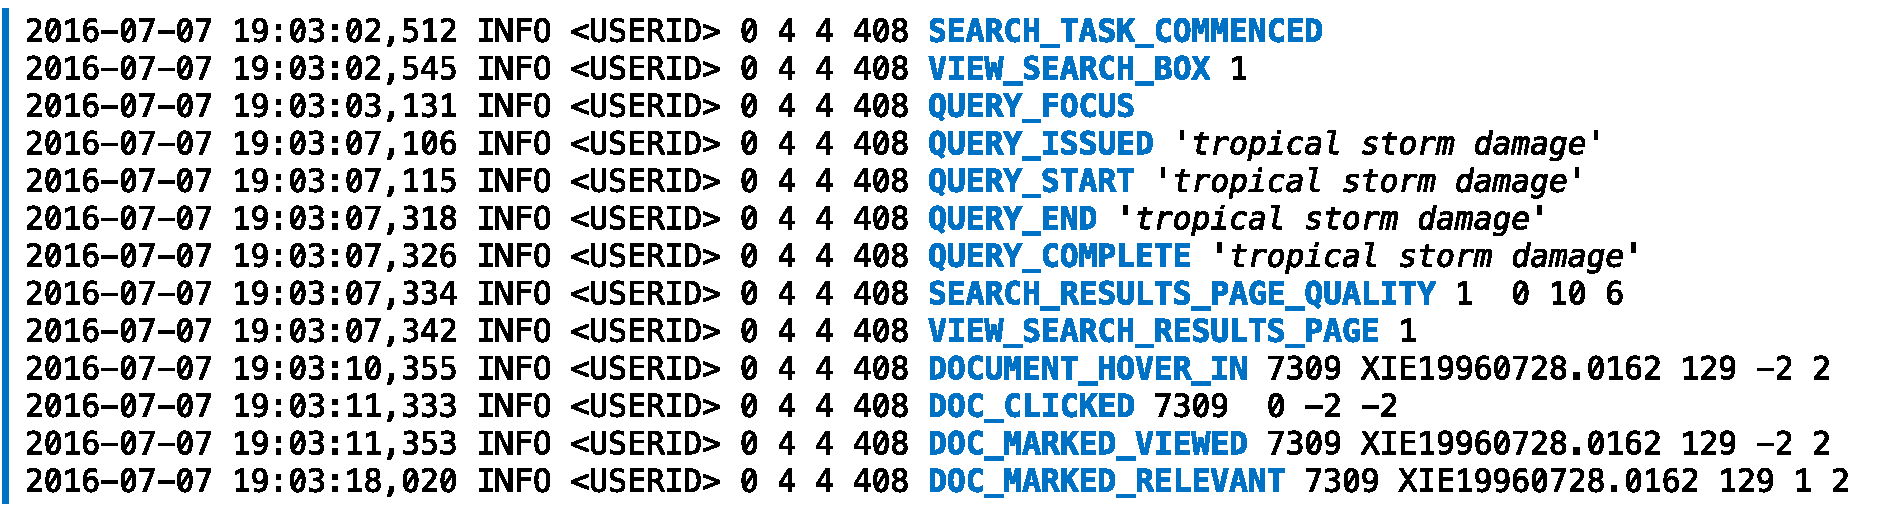
\includegraphics{figures/ch6-log.pdf}}
    \caption[Experiment log file excerpt]{An excerpt from the snippets user study, as detailed in Chapter~\ref{chap:snippets}. This example provides a sequence of interactions that were logged by the \treconomics~framework.}
    \label{fig:log}
\end{figure}

In addition to the interaction log, the \treconomics~framework also saved the responses from surveys as filled in by the subjects of each study. These were saved to a separate~\gls{acr:rdbms}, with a number of scripts subsequently created to extract and analyse the saved responses.

\subsection{Crowdsourcing Considerations}\label{sec:csm:methodology:user:crowdsourcing}
An important factor in planning any user study is the economics of collecting input from subjects. \emph{Where do the subjects come from? How do we recruit them?} A traditional, lab-based study as discussed in Section~\ref{sec:ir_background:user} typically involves a significant investment in time and monetary cost from the researchers conducting the experiment~\citep{spool2001testing}. For both user studies previously detailed, we employed a \emph{crowdsourced} approach to our experimentation. Crowdsourcing is the practice of obtaining input into a task by enlisting the services of a number of people, recruited over the Internet.

As highlighted by Zuccon et al.~\cite{zuccon2013crowdsourcing_comparisons}, crowdsourcing provides an alternative means for capturing user interactions and search behaviours. Greater volumes of data can be obtained from more heterogeneous workers at a lower cost -- all within a shorter timeframe. Of course, pitfalls of a crowdsourced approach include the possibility of workers completing tasks as efficiently as possible, or submitting their tasks without performing the requested operations~\citep{feild2010turkers}.

Despite these issues, it has been shown that there is little difference in the quality between crowdsourced and lab-based studies~\cite{zuccon2013crowdsourcing_comparisons}. Nevertheless, quality control is a major component of a well-executed crowdsourced experiment~\cite{bota2016information_cards}. Employing crowdsourcing for our two user studies, we detail in the remainder of this section the precautions that were taken during, discussing both the requirements for the subjects and their technical setup -- as well as a discussion of the crowdsourcing platform used.

\subsubsection{Platform Details}
Both studies were run over the \emph{Amazon Mechanical Turk (MTurk)} platform. Workers\footnote{In this section, a \emph{worker} refers to an individual undertaking the experiment on the MTurk platform. This term is considered interchangeable with a \emph{subject.}} from the platform each performed a single task (or, to use MTurk language, a \emph{Human Intelligence Task (HIT)}), with a single HIT corresponding to the entire experiment. This is in contrast to many HITs, where workers would typically undertake small, typically decision-based, transactions (for an example of such a study where this took place, refer to~\cite{bota2016information_cards}).

\subsubsection{Subject Requirements}
Due to the expected length that workers would take to complete the two studies\footnote{Note that two different sets of workers were used -- the studies were run at different times.}, workers who completed the study in full were reimbursed for their time with US\$9 -- greater than the hourly minimum wage set by the US federal government. Workers interested in undertaking each of the two studies were required to meet a certain minimum set of criteria to be eligible to participate. We required that workers were:

\begin{itemize}
    \item[\emph{(i)}]{from the United States;}
    \item[\emph{(ii)}]{native English speakers;}
    \item[\emph{(iii)}]{possessed a HIT acceptance rate of at least 95\%; and}
    \item[\emph{(iv)}]{had at least had 1000 prior HITs approved.}
\end{itemize}

Requiring \emph{(iii)} and \emph{(iv)} reduced the likelihood of recruiting workers who would not complete the study in a satisfactory manner. Recruits were forewarned about the length of the HIT, providing them with a chance to abandon the experiment if they felt the expected time was too long.

\subsubsection{Technical Requirements}\label{sec:csm:methodology:user:crowdsourcing:technical}
Given worker limitations, we also enforced a number of technical constraints. Workers attempting each experiment were required to have a sufficiently large computer screen to display the experimental interface without having to resort to excessive scrolling, and ensured a consistent number of result summaries would be present on different worker's screens. As such, we imposed a minimum display resolution of $1024x768$ for both studies. Conducted through a web browser, we wanted to ensure that only the controls provided by the experimental apparatus were used, meaning that the popup window that we highlighted in Section~\ref{sec:csm:methodology:user:interface} had all other browser controls disabled to the best of our ability (i.e. browser history navigation, etc.). The experimental system was tested on several major web browsers, across different operating systems. This gave us confidence that a similar experience would be had across different system configurations.

\section{Extracting User Study Data}\label{sec:csm:methodology:extracting}
As discussed in Section~\ref{sec:csm:methodology:user:capturing}, the \treconomics~framework provided the necessary infrastructure for us to log the various interactions and capture survey responses from each individual subject across the two user studies trialled. In this section, we provide details on the different aspects that we subsequently used to evaluate searcher behaviours, performance and user experience. Figure~\ref{fig:evaluation_methodology} provides a graphical illustration of how we split the various aspects we consider into four distinct categories.

The first three categories can be extracted directly from the interaction log that recorded different interactions by each subject as they progressed through the experiment. The categories we considered are listed below.

\begin{itemize}
    
    \item[]{\blueboxbold{Behavioural Measures} capture the broad interactions that take place, such as the number of documents that a searcher examined in detail.}
    \item[]{\blueboxbold{Performance} measures could be extrapolated, with aid of~\gls{acr:trec} QREL relevance judgements, to ascertain the performance of subjects.}
    \item[]{\blueboxbold{Time-Based} measures can also be derived from directly examining the interaction log, measuring the time spent between different logged interactions.}
    
\end{itemize}

In addition to these categories, we also observed a number of \blueboxbold{user experience} measures that are derived from a series of surveys that subjects were presented with as they were walked through the experimental process. In particular, as highlighted in Section~\ref{sec:csm:methodology:user:flow}, surveys were presented to subjects at a number of different stages throughout the experiment. In conjunction with the three log-based categories defined above, the user experience measures could be used to complement the empirical evidence to see whether the interactions of subjects actually correlated with their perceived experiences.

In all, the interactions -- including aspects such as clicks, and time-based measures, were used as a \emph{grounding} for our subsequent user simulations. These are discussed in Section~\ref{chap:csm:method:simulation} and derived for each experimental condition and interface trialled.

\begin{figure}[t!]
    \centering
    \resizebox{1\hsize}{!}{
    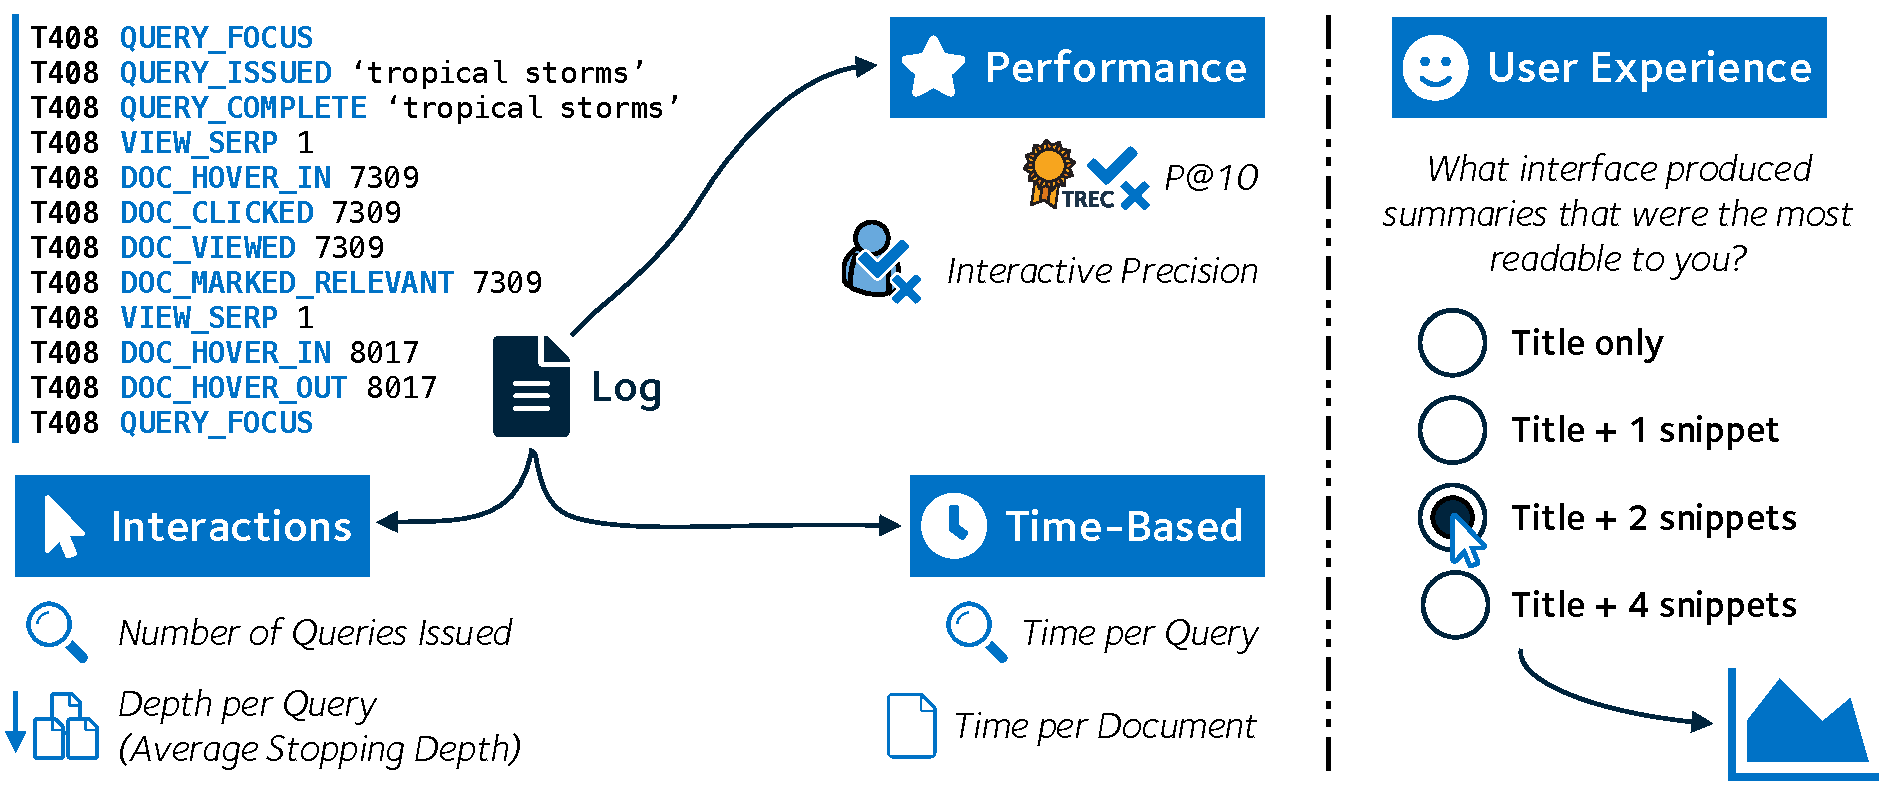
\includegraphics{figures/ch4-evaluation.pdf}}
    \caption[Examples of Evaluation Measures]{An illustration of the different types of measures that are captured, and from what sources. Interaction, time-based and performance measures are derived from the user study experiment log (with~\gls{acr:trec} QRELs used in conjunction with the interaction log to compute a subject's performance). User experience metrics are collated from a number of different surveys. Refer to Section~\ref{sec:csm:methodology:extracting} for more information.}
    \label{fig:evaluation_methodology}
\end{figure}

\subsection{Behavioural Measures}
Recorded solely from interaction log data, the basic interactions covered a large proportion of the aspects we considered in our analyses. They key behavioural measures we examined were:

\begin{itemize}
    \item{the number of \blueboxbold{queries issued};}
    \item{the number of \blueboxbold{documents viewed};}
    \item{the number of \blueboxbold{\glsplural{acr:serp} viewed}; and}
    \item{the \blueboxbold{depths} to which subjects clicked on (and hovered over), regarding the result summaries presented on the~\glsplural{acr:serp}.}
\end{itemize}

From these measures, we could then ascertain whether searcher behaviour varied when a certain condition or interface was changed -- allowing us to address questions such as \emph{whether snippet length affects the depth to which searchers examine content?} To compute depths, click and hover depths were used -- we however only report click depths in subsequent contributory chapters. The reasoning for this is discussed in Section~\ref{sec:csm:methodology:extracting:time} below. These measures were observed over each query issued by subjects.

% -- we could then take an average for each subject. We could go even further, too -- averaging over each topic, interface or condition as required to observe any notable trends in behavioural changes.

\subsection{Time-Based Measures}\label{sec:csm:methodology:extracting:time}
As discussed in Section~\ref{sec:csm:methodology:user:capturing} -- and also illustrated in Figure~\ref{fig:log} on page~\pageref{fig:log}, each logged interaction was saved with a timestamp which allowed us to determine when each event occurred.\footnote{Timestamps were saved to the nearest thousandth of a second, as per the specification of the standard Python logging framework -- refer to \url{https://docs.python.org/2/howto/logging-cookbook.html} \urlaccessed{2018-05-29} for an example of the framework in action.}. With these timestamps, we could then measure the time between two associated events, thus yielding the time taken to perform a given activity. We considered five key time-based measures across both user studies, namely:

\begin{itemize}
    \item{the time spent \blueboxbold{issuing queries};}
    \item{the time spent examining the \blueboxbold{content on~\glsplural{acr:serp}};}
    \item{the time spent examining \blueboxbold{individual result summaries};}
    \item{the time spent examining \blueboxbold{documents}; and, of course}
    \item{the summation of all of the above to yield the \blueboxbold{total session time}.}
\end{itemize}

It should be noted that in this thesis, \blueboxbold{we report all durations in seconds}. Event durations from the interaction log could be calculated in a relatively straightforward fashion. For example, the duration between the \texttt{QUERY\_FOCUS} to \texttt{QUERY\_ISSUED} events yielded the subject's query time. We of course acknowledge that in all likelihood, subjects may have considered what query to issue before focusing on the query box. However, we did not have the tools at our disposal to measure this. 

One further point worthy of note was how we computed the time spent examining each result summary. The per result summary time was approximated by taking the total time spent on a given~\gls{acr:serp}, and dividing that value by the click depth that was reached on that~\gls{acr:serp}. This was originally computed by summing up the time spent hovering over results with the subject's mouse cursor, as this was shown in prior studies to correlate strongly with the user's gaze on the screen~\citep{chen2001mouse_cursor, smucker2014judging_relevance_movements}. However, issues with network latency meant that several of the hover events were logged in the incorrect order, making such an approach unviable. Using the click depth and total~\gls{acr:serp} time provided us with an approximation with which to work with. However, the approximation also makes an assumption that subjects examined each result summary on a~\gls{acr:serp}, up until a particular depth, for an equal period of time. This was sufficient for the work in our study to ascertain whether or not a variation in the task goal or presentation of results affected search depths.

\subsection{Performance Measures}\label{sec:csm:methodology:extracting:performance}
As previously discussed, we were also able to extract a number of different performance measures from the interaction logs, too. Using the raw data from the logs, we could then, in conjunction with our set of~\gls{acr:trec} QRELs, compute a number of performances measures.\footnote{Some measures were computed with the \texttt{trec\_eval} evaluation tool, discussed in Section~\ref{sec:ir_background:basics:cranfield:trec}.} Key performance measures that we captured included:

\begin{itemize}
    \item{the \blueboxbold{overall performance of queries}, measured with \blueboxbold{P@10}; and}
    \item{\blueboxbold{interactive precision and recall} (as discussed in Section~\ref{sec:ir_background:user:evaluation:interactive_pr}), including:}
    
    \begin{itemize}
        \item{the number of documents saved (identified as relevant); and}
        \item{the number of those documents that were~\gls{acr:trec} relevant (and vice-versa).}
    \end{itemize}
\end{itemize}

\blueboxheader{Grounding Subsequent Experiments} With behavioural measures and time-based measures in particular, these could be then used to \emph{ground} subsequent experiments. Refer to Section~\ref{chap:csm:method:simulation:grounding} for further information on how this was achieved. The above measures are however sufficient for analysing how searcher behaviour changed under different contexts.

\subsection{Demographics and User Experience Surveys}\label{sec:csm:methodology:extracting:user}
A number of surveys, as discussed in Section~\ref{sec:csm:methodology:user:capturing}, were also filled out by subjects capturing a variety of information about their search experiences. While there are similarities between what is asked (refer to Chapters~\ref{chap:snippets} and~\ref{chap:diversity} for further details), we in this section provide a high-level overview of the different surveys, before examining questions that were common between the two. We break these overviews into three sections, in the order of the experimental flow detailed in Section~\ref{sec:csm:methodology:user:flow} -- demographics, pre- and post-task surveys, and post-experiment surveys.

\subsubsection{Demographics}
Details in keeping with general demographics were attained about the different subjects from this survey. These included the subject's age, gender and occupation. We also queried the subject on their highest level of professional qualification (e.g. high school, Honours, MSc or PhD). A number of questions were also asked about their perceived proficiency and approach to searching for information on the~\gls{acr:www}. Questions included how often they searched for information, what pointing device they were using (i.e. mouse, trackpad), and their preferred web search engine. Finally, given that both experiments considered news search, we asked how often the subjects searched for news articles online.

\subsubsection{Pre-Task}
Between both user studies, we asked the same questions within the pre-task survey. Subjects were provided with a short description of their search task and a topic description, providing their information need for said task. After examining the topic description, subjects were then queried on the following:

\begin{itemize}
    \item{how well they knew about the topic prior to this study;}
    \item{how relevant the topic was to their life;}
    \item{how interested they were to learn more about the topic;}
    \item{whether they had searched for information related to the topic before; and}
    \item{how difficult they felt it would be to search for information on the topic before commencing.}
\end{itemize}

Responses were provided on a five-point scale, providing the option for neutrality between the two extremes -- extremes being \emph{nothing/not at all/very difficult} to \emph{lots/very much/very easy.} Responses to these questions helped us gauge the perceived difficulty of the task, and ascertain how much background knowledge could potentially affect results.

\subsubsection{Post-Task and Post-Experiment}
Post-task and post-experiment surveys were unique to each of the two user studies. Chapters~\ref{chap:snippets} and~\ref{chap:diversity} provide further information on what questions were asked. However, the post-task surveys focused on how well the subjects thought they (and the retrieval system, under the given condition and/or interface) performed during the search task. Post-task surveys considered the experiment as a whole, asking questions about what condition and/or interface the subjects preferred, or performed more to their liking, for example.

\section{Simulating Searcher Behaviours}\label{chap:csm:method:simulation}
With the general layout and components of the two user studies explained, we now consider how we \emph{simulated searcher behaviours.} Highlighted in Section~\ref{sec:ir_background:user:simulation}, simulation provides a low-cost means for exploring a variety of different searcher strategies and configurations. In this section, we provide an overview of the general aspects of the \blueboxbold{stochastically-based} searcher simulations that we discuss the results of in subsequent chapters of this thesis. Specifically, we discuss in this section:

\begin{itemize}
    \item{how our simulations were \emph{grounded;} and}
    \item{how we instantiated the different components of the~\gls{acr:csm} defined in Chapter~\ref{chap:csm} for our simulation experiments.}
\end{itemize}

We conclude the chapter with a discussion as to how we evaluate the results from our simulations, allowing us to determine what stopping strategies offer the best overall performance and approximations of real-world searcher behaviours. This is done in consideration of the two user studies discussed in Chapters~\ref{chap:snippets} and~\ref{chap:diversity}. By grounding our simulations with data derived from the two aforementioned user studies, we can then obtain an insight into how searcher stopping behaviours varies under different contexts.

\blueboxheader{The Mean Searcher} Comparisons between simulations and real-world searcher approximations are made between the \emph{average} behaviours observed. This average behaviour is considered across each of the different experimental interfaces and conditions that we trial across the two user studies, discussed in Chapters~\ref{chap:snippets} and~\ref{chap:diversity}. This consideration: \emph{(i)} simplifies and reduces the number of simulations that are required to be run; and \emph{(ii)} provides a simple overview of how stopping behaviour varies across each interface and condition, rather than across each individual searcher.

\blueboxheader{Considering Stochastic Simulations} As eluded to above, we consider in this thesis a series of different \emph{stochastically-based} simulations that attempt to mimic searcher behaviours. Currently, a majority of research that considers the simulation of interaction are also stochastic in nature, utilising probabilistic models. For example,~\cite{carterette2011effectiveness_evaluation} simulated the interaction of users for the purposes of evaluation through a dynamic test collection. While not explicitly stated, the underlying model of their simulations followed a similar process to the~\gls{acr:csm} as described in Chapter~\ref{chap:csm}, and were instantiated with probabilistic components.~\cite{baskaya2013behavioural_factors}, as discussed in Section~\ref{sec:stopping_background:models:conceptual:simple}, developed a Markov-based model of the search process, with changes in state determined by a series of different probabilities. A similar, probabilistic browsing model was also proposed by~\cite{yilmaz2010browsing_utility}. These models considered probabilistically determining, for instance, the attractiveness of a result summary to the given information need -- something that we also utilise. We discuss this further in Section~\ref{chap:csm:method:simulation:grounding:judgements}.

\blueboxheader{The SimIIR Framework} All simulations that were run as part of this thesis were done so using the \simiir~framework, a custom built framework for the simulation of interaction within the~\gls{acr:iir} process.\footnote{\simiir~can be accessed at \url{https://github.com/leifos/simiir}. \urlaccessed{2018-05-29}} As outlined in Chapter~\ref{chap:intro}, the \simiir~framework is in effect is one of the major contributions offered by this thesis. The~\gls{acr:csm}, as outlined in Chapter~\ref{chap:csm}, is implemented within the framework and offers a high level of customisability in order to trial various different component configurations.~\cite{maxwell2016simiir} provides an overview of the framework.

\subsection{Grounding and Instantiating Simulations}\label{chap:csm:method:simulation:grounding}
Repeated many times throughout this thesis so far, the \emph{grounding} of simulations is crucial for ensuring their overall credibility~\citep{azzopardi2010workshop}. Simulations that are not properly grounded with data from real-world observations means that results would then be questionable. As such, this is an area that was taken seriously during the design of our methodology. After consideration of the~\gls{acr:csm}, we considered grounding from three key perspectives:

\begin{itemize}
    \item{the generation of pseudo-realistic \blueboxbold{queries} to issue to the underlying Whoosh search engine (refer to Section~\ref{sec:csm:methodology:collection});}
    \item{the consideration of various \blueboxbold{interaction costs}; and}
    \item{the inclusion of various \blueboxbold{interaction probabilities} for determining relevancy.}
\end{itemize}

These are considered in conjunction with our aforementioned stopping strategies (refer to Chapter~\ref{chap:strategies}), and imposed constrained on the session for each simulated searcher. The remainder of this section discusses each of the key components of our simulations, and how we instantiated them to produce realistic, credible simulations of interaction.

\subsubsection{Interaction Costs}\label{chap:csm:method:simulation:grounding:costs}
Upon the examination of the~\gls{acr:csm}, illustrated in Figure~\ref{fig:csm} on page~\pageref{fig:csm}, a number of different \emph{interaction costs} can be derived. These are costs that must be expended by searchers subscribing to the model, in order for them to successfully complete the search process. We identified five different interaction costs that searchers are faced with. The five different interaction costs are:

\begin{itemize}
    \item{the time taken to \blueboxbold{issue a query} to the underlying search engine;}
    \item{how long a searcher will spend \blueboxbold{examining a~\gls{acr:serp}}, using the time to judge whether the contents of the~\gls{acr:serp} should be examined in more detail, or abandoned altogether;}
    \item{the time taken to \blueboxbold{examine an individual result summary} in depth;}
    \item{the amount of time required to \blueboxbold{examine a document} in full; and}
    \item{the time taken for determining whether a \blueboxbold{document should be saved as relevant}.}
\end{itemize}

Costs, measured in seconds, are averaged over each different condition and interface trialled between the two different user studies discussed in Chapters~\ref{chap:snippets} and~\ref{chap:diversity}. Refer to these chapters for tables of the actual interaction costs that were extracted from the interaction log data.

\blueboxheader{Extracting Interaction Costs}
To extract interaction costs for each interface and condition, we followed the same approach as discussed in Section~\ref{sec:csm:methodology:extracting:time} for extracting time-based measures. For each of the five interaction costs, we measured the time difference between two different logged events, before computing an average. Below, we outline the key events that we used to measure each of the five interaction costs. The interaction costs are also illustrated in Figure~\ref{fig:costs}.

\begin{figure}[t!]
    \centering
    \resizebox{1\hsize}{!}{
    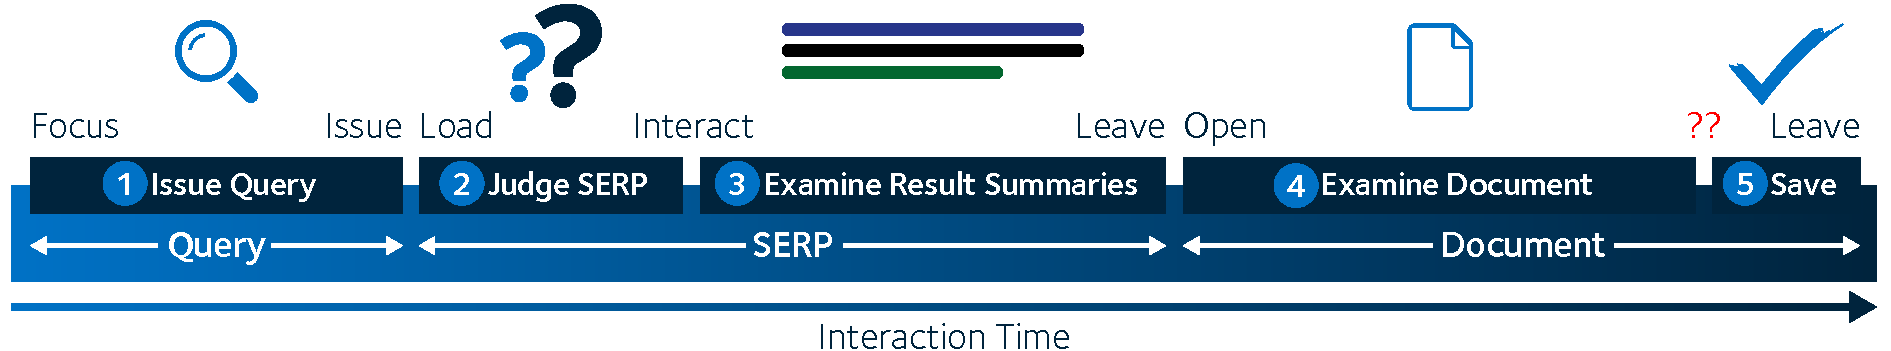
\includegraphics{figures/ch6-costs.pdf}}
    \caption[Interaction costs]{Illustration of the five interaction costs paid by searchers subscribing to the~\gls{acr:csm}. Each cost is shown with the start and end events, by which the costs were measured from the user study interaction logs. Time spent on individual components is shown in white. Refer to Section~\ref{chap:csm:method:simulation:grounding:costs} for a detailed explanation of each interaction cost considered.}
    \label{fig:costs}
\end{figure}

\begin{itemize}
    \item{\blueboxbold{1 (Querying)} As discussed in Section~\ref{sec:csm:methodology:extracting:time}, querying is measured from when the subject focused on the query box, to the point where they submitted the query.}
    \item{\blueboxbold{2 (\gls{acr:serp} Examination)} For this particular cost, we assumed that searchers would spend time judging the overall quality of the~\gls{acr:serp} from the point at which the~\gls{acr:serp} is rendered on their screen, to the point where they begin interacting with it in any way.}
    \item{\blueboxbold{3 (Result Summary Examination)} Considering the difficulties in estimating the depth to which subjects hovered over result summaries (discussed in Section~\ref{sec:csm:methodology:extracting:time}), we again used the click depth to estimate result summary examination times.}
    % This was achieved by taking the point at which a searcher began interacting with a~\gls{acr:serp}, to the point that they left it. This time was then divided by the subject's click depth for that particular~\gls{acr:serp}, yielding the estimation used.
    \item{\blueboxbold{4 (Document Examination)} This cost was determined by measuring the difference between the point at which a requested document was displayed on the subject's screen, to the point at which they left it.}
    \item{\blueboxbold{5 (Saving a Document)} \todo{The final interaction cost considered the time from which a searcher did x, to when they did y.}}
\end{itemize}

As can be seen from the discussion above, determining some interaction costs (e.g. querying) are more straightforward than others. For the~\gls{acr:serp} examination interaction and result summary interaction costs in particular, key assumptions are made considering evidence from prior studies, showing that the movements of the mouse cursor on the subject's computer screen correlate strongly with their gaze~\citep{chen2001mouse_cursor, smucker2014judging_relevance_movements}. In addition, \todo{the user interface illustrated in the right screenshot in Figure~\ref{fig:interfaces} on page~\pageref{fig:interfaces} shows that saving a document involves only the click of a button, we argue that a period of additional time must be spent to do what. As such, this is why we consider the last interaction cost listed above.}

\blueboxheader{Fixed Interaction Costs}
All simulations discussed in this thesis rely on the notion that all interaction costs are \emph{fixed} over each interface and condition trialled. This decision was primarily chosen to reduce the complexity of our simulations. By including dynamic interaction costs, this would have made the simulations themselves -- and the subsequent comparisons -- much more complex. We do acknowledge this as a limitation of our work, as a searcher should take considerably less time to judge a document consisting of two paragraphs than a document consisting of 20. We also acknowledge the existence of measures such as \emph{time-biased gain}~\citep{smucker2012tbg} that would allow for such an estimation of cost to be made.

\subsubsection{Query Generation Strategies}\label{chap:csm:method:simulation:grounding:querying}
The \emph{generation of queries} is an important aspect of any simulation of interaction. From the simplistic~\gls{acr:trec}-style model of search where a single query is issued (refer to Section~\ref{sec:stopping_background:models:conceptual:trec}), numerous studies have focused upon the issue of query generation, and how one can generate a series of pseudo-realistic queries. We discuss these prior works in Section~\ref{sec:ir_background:user:simulation}.

However, we consider a number of different \emph{querying strategies} as proposed by~\cite{keskustalo2009querying} and~\cite{baskaya2013behavioural_factors} in order to generate queries for our simulations. These strategies are considered to be \emph{idealised, prototypical} approaches to query generation, being grounded from a prior user study examining the query behaviour of subjects.\footnote{Refer to~\cite{keskustalo2009querying} for further information on the user study undertaken.}

Of the five strategies identified by the authors, we consider two in this thesis that were shown in subsequent simulations by~\cite{keskustalo2009querying} to yield the worst and best performance. The two querying strategies, named as \blueboxbold{QS1} and \blueboxbold{QS3}, are briefly explained below. We also provide an illustration of the two strategies in Figure~\ref{fig:querying}, where $Q_n$ represents query $n$ within a search session, and $t_n$ represents query term $n$ from a list of terms available to formulate queries.

\begin{figure}[t!]
    \centering
    \resizebox{1\hsize}{!}{
    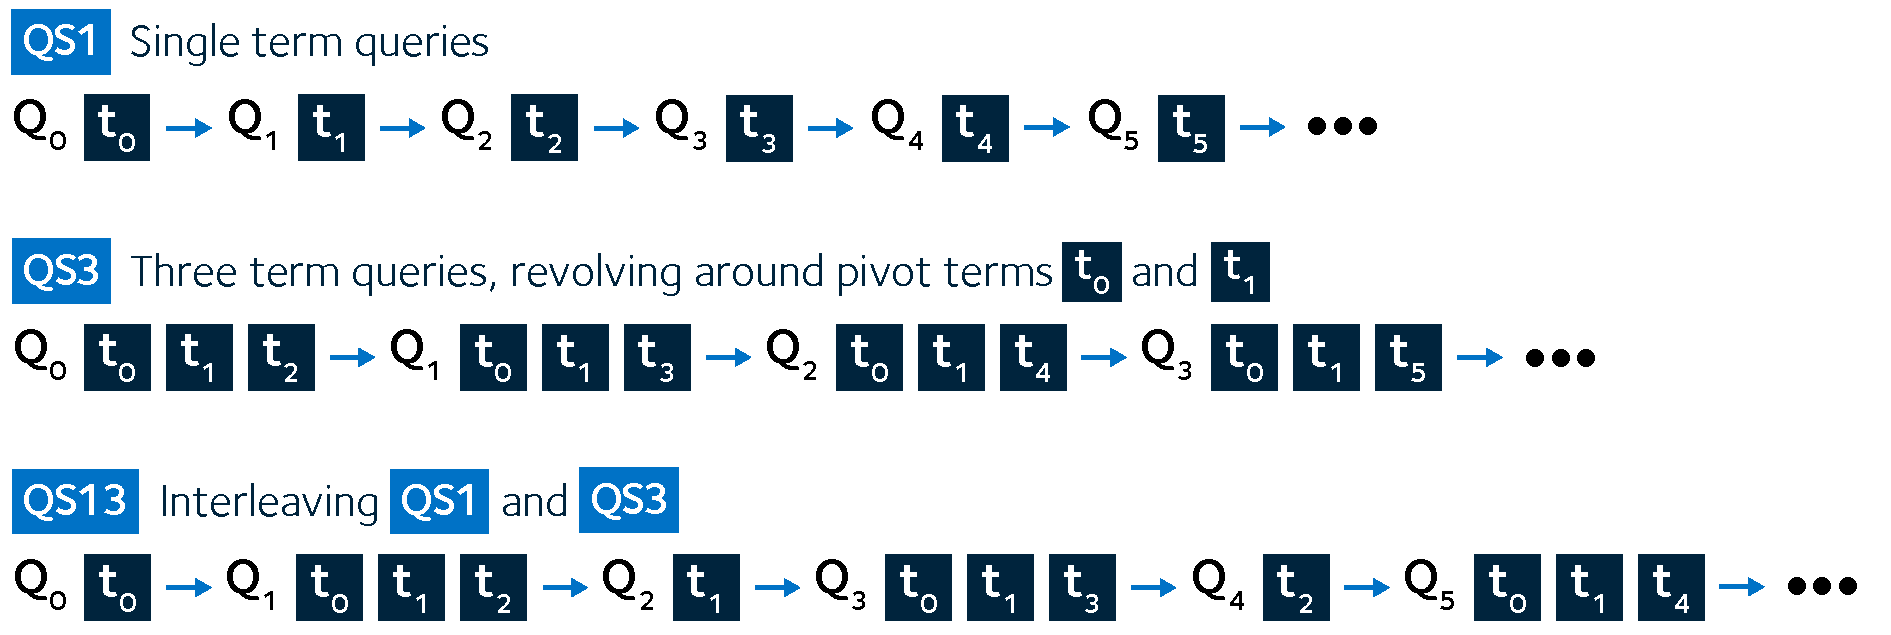
\includegraphics{figures/ch6-querying.pdf}}
    \caption[Query Strategies example]{Extensive examples of the four querying strategies used in this thesis, \blueboxbold{QS1}, \blueboxbold{QS3}, \blueboxbold{QS13} and \blueboxbold{QS13\textsuperscript{+}}. Queries are denoted by \emph{Q\textsubscript{n}}, with individual terms denoted by \darkblueboxbold{t\textsubscript{n}}. In these examples, a total of six terms are used (from \darkblueboxbold{t\textsubscript{0}} to \darkblueboxbold{t\textsubscript{5}}). Queries are separated by arrows (~
\includegraphics[height=\fontcharht\font`\d]{figures/src/arrow-blue-right.pdf}). The stop sign denotes a lack of further queries; at this point a searcher would have exhausted possible query combinations.}
    \label{fig:querying}
\end{figure}

\begin{itemize}
    \item{\blueboxbold{QS1 (Single Term)} This querying strategy generates a series of \emph{single term queries.}}
    \item{\blueboxbold{QS3 (Three Term)} This second querying strategy generates queries with two \emph{pivot} terms, and one other term. The first two terms therefore remain constant, with the third term changing for each subsequent query.}
\end{itemize}

These queries are relatively short, and are considered realistic in the sense that queries issued in real-life web search sessions consist three terms on average~\citep{keskustalo2009querying}.

With these two querying strategies in mind, we then combined them together to produce an \emph{interleaved querying strategy,} \blueboxbold{QS13}.

\begin{itemize}
    \item{\blueboxbold{QS13 (Interleaved)} With this querying strategy, queries from both \blueboxbold{QS1} and \blueboxbold{QS3} are generated, and subsequently interleaved between each other, starting with the first query from \blueboxbold{QS1}.}
\end{itemize}

Refer to Figure~\ref{fig:querying} for an example of how this strategy works. The idea behind this querying strategy is that it allows us to test the \blueboxbold{robustness} of the new~\gls{acr:serp} level stopping decision point and the various stopping strategies that we trial (our implementations of each are discussed in Sections~\ref{chap:csm:method:simulation:grounding:serp} and~\ref{chap:csm:method:simulation:grounding:stopping_strats} respectively). With~\cite{keskustalo2009querying} highlighting that \blueboxbold{QS1} yields relatively poor performance compare to~\blueboxbold{QS3}, it therefore follows that a searcher, when issuing a query generated by \blueboxbold{QS1}, will observe that the results presented are of poor quality, and thus stop at a comparatively shallower depth when compared to examining the results of queries issued by \blueboxbold{QS3}. Examining many results from a poor query is by and large a waste of the searcher's time.

Our final querying strategy, \blueboxbold{QS3\textsuperscript{+}}, is based upon the pivot term approach as seen by \blueboxbold{QS3}. Again, refer to Figure~\ref{fig:querying} for an example of how this strategy works.

\begin{itemize}
    \item{\blueboxbold{QS3\textsuperscript{+} (Realistic)} This final querying strategy builds up queries to three terms in length, using the two pivot terms as described before as a starting point.}
\end{itemize}

Previous work has shown that real-world searchers steadily build up the number of terms they used in their queries as they acquire more information. Short queries are issued initially, and the length then increases~\citep{keskustalo2009querying}. This is our rationale behind \blueboxbold{QS3\textsuperscript{+}}, and provides a more \blueboxbold{realistic} querying strategy with which to examine performance with. This is in conjunction with \blueboxbold{QS13} that allows us to test the robustness of the different stopping strategies and the~\gls{acr:serp} stopping decision point.

\blueboxheader{Reported Querying Strategies}
In this section, we introduced four different querying strategies -- two underlying strategies from the work by~\cite{keskustalo2009querying}, and two strategies based upon this prior work. The latter two allowed us to test the robustness and realism of the various simulation configurations. As such, the work in this thesis reports only on simulations that were run with \blueboxbold{QS13} and \blueboxbold{QS13\textsuperscript{+}}.

%To recap, the interleaving of good and bad queries poses a key challenge to the stopping components of the~\gls{acr:csm}: to spot a poor performing query and subsequently stop early, thus saving time.

\blueboxheader{Term List Generation}
Each of the querying strategies above are dependent upon a series of ranked terms from which queries can be created. This was achieved by first taking the \gls{acr:trec} title and description for a given topic, and creating a \emph{Maximum Likelihood Estimate (MLE)} language model (as discussed in Section~\ref{sec:ir_background:basics:models:language}), allowing us to create a probability distribution for the likelihood of a term to appear in a topic description, i.e. $p(term|topic)$. Considering our first underlying querying strategy \blueboxbold{QS1}, we could then extract a list of single terms, ranked according to $p(term|topic)$. This provided the list of terms from which queries could be generated. Our approach to pivot term-based \blueboxbold{QS3} was more complex. Taking the title terms exclusively, we then took all possible two-term combinations of the title terms, and selected the pair with the highest joint probability to act as the two pivot terms for the querying strategy. A list of candidate queries, $q$, could then be constructed by appending another term from the topic to the pivot terms (from both the topic title and description). These three term queries were then ranked according to $p(q|topic)$, yielding the final list of queries to be issued.

\subsubsection{Summary and Document Decision Making}\label{chap:csm:method:simulation:grounding:judgements}
Previously discussed in Section~\ref{chap:csm:method:simulation}, our simulations were stochastic in nature, with the decisions pertaining to the \blueboxbold{attractiveness of a result summary} \emph{(should I click this link and examine it further?)} and the \blueboxbold{relevancy of a document} to the given information need \emph{(should I save this document?)} determined through a series of different interaction probabilities. As we consider each interface and condition trialled separately, Chapters~\ref{chap:snippets} and~\ref{chap:diversity} present the interaction probabilities that were actually used within the simulations. In this section, we describe the approach used to derive them.

Like in previous studies considering the simulation of interaction -- such as those by~\cite{yilmaz2010browsing_utility} and~\cite{baskaya2013behavioural_factors}, for instance -- result summary and document decision making revolve around two key probabilities:

\begin{itemize}
    \item{the probability \blueboxbold{P(C)} of considering a given result summary on a~\gls{acr:serp} to be sufficiently attractive to \emph{`click'} and load the associated document; and}
    \item{the probability \blueboxbold{P(S)} of determining the document to be relevant to the given information need after examination, and thus \emph{saving} it.}
\end{itemize}

These are considered separately as the action of requesting a document from clicking on the associated result summary does not necessarily mean that the document \emph{is} relevant; merely, it means it appears attractive enough to examine in more detail~\citep{turpin2009summaries}. The above probabilities are broken down further with regards to~\gls{acr:trec} relevance. This entails examination of the~\gls{acr:trec} relevance judgements as discussed in Section~\ref{sec:csm:methodology:collection}, determining whether the result summary and/or document being clicked and/or saved was considered to be relevant to the given topic by the~\gls{acr:trec} assessors. As such, $P(C)$ and $P(S)$ can be split further, such that we can then determine:

\begin{itemize}
    \item{the probability that a result summary clicked is~\gls{acr:trec} relevant \blueboxbold{P(C|R)} or not \blueboxbold{P(C|N)}; and}
    \item{the probability that a document saved is~\gls{acr:trec} relevant \blueboxbold{P(S|R)} or not \blueboxbold{P(S|N)}.}
\end{itemize}

Taking these explanations, we could then take the interaction logs from the two user studies, split the interactions by the interface or condition that probabilities were to be derived for, and summate different measures -- as shown by the equation for calculating $P(C)$:

\begin{equation*}
    P(C) = \frac{|clicked_{Rel}| + |clicked_{\neg Rel}|}{|hovered_{Rel}| + |hovered_{\neg Rel}|};
\end{equation*}

and $P(S)$:

\begin{equation*}
    P(S) = \frac{|saved_{Rel}| + | saved_{\neg Rel} |}{|clicked_{Rel}| + |clicked_{\neg Rel}|}.
\end{equation*}

In the above equations, $Rel$ denotes the count for~\gls{acr:trec} relevant items, with $\neg Rel$ representing items that were not~\gls{acr:trec} relevant. Finally, $|clicked|$ represents the number of result summaries that were clicked (deemed attractive enough to examine further), $|hovered|$ denotes the number of result summaries that a subject hovered over with their mouse, with $|saved|$ denoting the number of documents that were identified as relevant, and subsequently \emph{saved.} To compute probabilities concerning~\gls{acr:trec} relevance only (i.e. $P(C|R)$ and $P(S|R)$), $\neg Rel$ elements were removed, with $Rel$ elements being removed for computing probabilities of interaction for items that were not~\gls{acr:trec} relevant (i.e. $P(C|N)$ and $P(S|N)$).

Like in Section~\ref{sec:csm:methodology:extracting:time}, the number of hovered result summaries was inferred due to issues with collecting actual hover events. To calculate the hover counts, we obtained the subject's greatest click depth for a given~\gls{acr:serp}, and summed up to that point. For example, if a subject clicked a document at a depth of $7$, the hover depth was assumed to be as such.

\blueboxheader{Stochastic Simulations}
This stochastic approach to modelling interactions provides a simple means of operationalising the components of the simulation that attempt to judge the attractiveness and relevancy of result summaries and documents, respectively.\footnote{This is not to say that stochastic approach is the only way the model such a process. For example,~\cite{maxwell2016agents} considered a \emph{deterministic} approach. A classifier was trained that then allowed a \emph{simulated agent} to deterministically decide the attractiveness of a result summary, for example.}

However, such an approach is not without limitation. By their very nature, a stochastic simulation, based upon random probabilities, will require a large number of different trials to be executed from which an \emph{average} can be formed. Each trial will potentially result in a different outcome -- perhaps, for example, with fewer documents marked in a second trial than compared to the first. This leads to a huge variance between different trials, which in turn leads to a requirement of running a large number of trials, such \emph{Monte-Carlo style simulations}~\citep{benov2016manhattan}. This in turn leads to huge increases in the amount of time required to run all simulations, as well as the computational power required.

\blueboxheader{Pre-Rolled Judgements}
To mitigate this issue, we used a series of so-called \emph{pre-rolled judgements.} This ensured that we could provide a fair comparison between configurations, whilst reducing the number of runs required to reach a point at which the simulations converged. For each document within the AQUAINT collection used, we pre-computed the various probabilities, storing them in \emph{action judgement files,} with one related to result summaries (i.e. $P(C)$), and the other related to saving documents (i.e. $P(S)$). If a document was judged to be relevant in one run, then by pre-computing these actions in advance, the same document would then be considered to be relevant in other runs.

This process was repeated ten times using different seeded values for each run. This meant that for every different simulated searcher configuration (i.e. considering stopping strategies, etc.), we ran a total of ten trials in which documents could be marked as either relevant or non-relevant. This meant, as previously mentioned, a fairer and paired comparison could be undertaken within runs. This subsequently also means that for each run, all results reported later in this thesis are the average over all ten trials. \todo{do validation simulation too}

\subsubsection{Computing Gain}\label{chap:csm:method:simulation:grounding:gain}
As searchers examine information, they \emph{gain knowledge} that helps shape their mental model of the underlying information need~\citep{nickles1995judgment}. While other works have focused upon this issue in depth, such as the work by~\cite{baskaya2013behavioural_factors}, we consider gain from a relatively simple standpoint. This keeps the complexity of our simulations manageable.

Gain is acquired when a simulated searcher, having determined to examine a document for relevance, considers it to be relevant, and subsequently \emph{saves} said document. During post-hoc analysis, we then can compute how many documents were saved and were~\gls{acr:trec} relevant. These are determined by examining the~\gls{acr:trec} relevancy judgements. The gain for the document is then simply computed as the relevancy judgement score from the~\gls{acr:trec} QRELs. Given that we utilised the~\gls{acr:trec} 2005 Robust Track~\citep{voorhees2006trec_robust}, \emph{graded relevance judgements} are used, as discussed in Section~\ref{sec:ir_background:user:evaluation:cg}. In essence, this value, when summated over all saved documents, is the \blueboxbold{Cumulative Gain (CG)} score for a simulated trial. This is discussed in more detail in Section~\ref{chap:csm:method:sim:runs}.

\blueboxheader{Gaining Elsewhere}
The means by which gain is computed in the work detailed in this thesis provides a further assumption. Gain can only be accrued from examination of a document, and subsequently saving it. This is not to say that in the real-world, searchers will not accrue gain from examination of other components, such as the result summary. This is particularly prevalent in the concept of \emph{good abandonment}~\citep{li2009good_abandonment}, where a searcher will abandon a~\gls{acr:serp} if he or she is satisfied by simply examining the information provided within result summaries, for example. We do not consider this within our simulations to simplify how gain is computed.

\subsubsection{\gls{acr:serp} Level Decision Making}\label{chap:csm:method:simulation:grounding:serp}
Previously outlined in Section~\ref{sec:csm:new_stopping}, the~\gls{acr:csm} includes an additional~\gls{acr:serp} level stopping decision point. Motivated by the \emph{information scent}\footnote{To recap, we discuss the notion of information scent in Section~\ref{sec:stopping_background:models:theoretical:ift}.} offered by a~\gls{acr:serp} (or \emph{patch}), this stopping point joins other established decision points, including snippet and session level stopping. The new decision point permits a searcher subscribing to the~\gls{acr:csm} to either \emph{enter} the~\gls{acr:serp} and begin examining result summaries in detail (if the~\gls{acr:serp}) appears to offer a good scent, or abandon the~\gls{acr:serp} if it appears to be poor, and thus save time. The remainder of this section discusses the various ways in which we implemented this new stopping decision point, allowing us to determine whether it leads to any improvements in overall search performance and better approximations to real-world searcher stopping behaviours.

\blueboxbold{Definition: Low vs. High Scent} First, we must define our interpretation of how the scent of a~\gls{acr:serp} was measured. We follow the work of~\cite{wu2014information_scent}, who stated that a page offering little or no relevant content could be considered to offer a low information scent. As such, our definition of a poor quality~\gls{acr:serp} is defined as $P@10=0.0$. We use this definition to delineate between \emph{good} and \emph{bad}~\glsplural{acr:serp} when considering interaction probabilities below.

\blueboxbold{Probability of Examination} For this new stopping decision point, we introduce the \emph{probability of examining a~\gls{acr:serp}}, or \blueboxbold{P(E)}. This determines how likely it is a searcher will \emph{enter} a~\gls{acr:serp} and begin to examine result summaries in detail. Taking this concept further, we can then consider two additional probabilities that incorporate the notion of a~\glsplural{acr:serp} information scent, yielding:

\begin{itemize}
    \item{\blueboxbold{P(E|HS)}, the probability of examining a~\gls{acr:serp} perceived to give a high information scent (i.e. a good quality~\gls{acr:serp}); and}
    \item{\blueboxbold{P(E|LS)}, the probability of examining a~\gls{acr:serp} offering what appears to be a low information scent (i.e. a poor quality~\gls{acr:serp}).}
\end{itemize}

\begin{figure}[t!]
    \centering
    \resizebox{1\hsize}{!}{
    
\includegraphics{figures/ch6-serp_probabilities.pdf}}
    \caption[Computing~\gls{acr:serp} examination probabilities]{A simple illustration highlighting how the different~\gls{acr:serp} examination costs were computed. We consider both the probability of examining~\glsplural{acr:serp} yielding both high and low information scents. Definitions are used from~\cite{wu2014information_scent} and~\cite{hassan2013serp_abandonment}.}
    \label{fig:serp_probabilities}
\end{figure}

These values were once again computed from interaction log data, derived from the two user studies discussed in Chapters~\ref{chap:snippets} and~\ref{chap:diversity}. As such, we do not report values for these probabilities here; rather, we discuss how we derived them. Refer to the specific chapters for specific values over each interface and condition trialled. Intuitively however, one would expect a searcher demonstrating competency at searching for information to know when a query is returning good results, and vice versa. As such, one would expect to see a higher probability for $P(E|HS)$ than when compared to $P(E|LS)$, and would thus provide evidence that searchers do indeed attempt to avoid low quality~\glsplural{acr:serp}.

As illustrated in Figure~\ref{fig:serp_probabilities}, we took each query issued from the interaction log, and extracted for each the $P@10$ score (as per~\cite{wu2014information_scent}). If $P@10=0.0$, the associated~\gls{acr:serp} for the query would have offered a low information scent. Conversely, if $P@10 > 0.0$, the information scent would have been considered to be high. For the interactions recorded on each~\gls{acr:serp}, we could then count the number that recorded no clicks (or no result summaries deemed to be attractive enough to examine further). We considered this as a definition of an \emph{abandoned~\gls{acr:serp}}, as used in previous work by~\cite{hassan2013serp_abandonment}. From these counts, we could then compute the probabilities of examining a~\gls{acr:serp}, as illustrated in Figure~\ref{fig:serp_probabilities}.

\blueboxbold{Considering Browser Viewport Size}
We now turn our attention to how a simulated searcher is able to make a judgement of the presented~\gls{acr:serp}. As we discussed previously in Section~\ref{sec:csm:new_stopping}, real-world searchers are able to infer the quality (and perhaps relevance) of a given page or~\gls{acr:serp} through the examination of various \emph{proximal cues}~\citep{chi2001information_scent}.

\begin{wrapfigure}[12]{r}{0.45\textwidth}
    \begin{center}
    \vspace*{-10mm}
    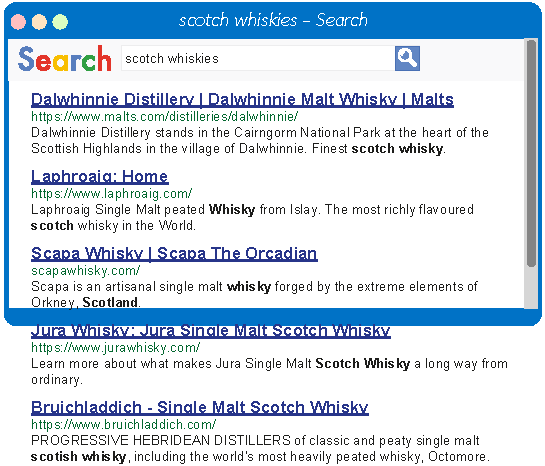
\includegraphics[width=1\textwidth]{figures/ch6-viewport.pdf}
    \end{center}
    \vspace*{-4mm}
    \caption[Viewport cutoff example]{The~\gls{acr:serp} viewport threshold. In this example, three result summaries are visible, with two not visible within the viewport. Therefore, \emph{v\textsubscript{size}=3}. Cheers!}
    \label{fig:viewport_cutoff}
\end{wrapfigure}

While we do not specifically examine different cues, instead relying on more simplistic means to operationalise the stopping decision point, we nevertheless do consider the \emph{size of the browser's viewport}. A~\gls{acr:serp} is typically larger than the viewport it is displayed within, which leads to the inclusion of scrollbars. We argue that a searcher can infer the quality of the~\gls{acr:serp} from the initial view they are presented with, and thus incorporate a \emph{viewport size} ($v_{size}$) variable in our implementations. A searcher can only judge what they can see. This variable can vary between the different interfaces we trialled -- for example, longer snippet text results in fewer result summaries being displayed in the initial view. By using a fixed-size popup window in the two user studies (as discussed in Section~\ref{sec:csm:methodology:user:interface}), we were then able to manually check the number of result summaries displayed within the popup window, and use these values to ground the new stopping decision point further.

\blueboxbold{Decision Point Implementations} We trialled three different implementations of the~\gls{acr:serp} level stopping decision point, providing us with the ability to determine the effect of incorporating it within the~\gls{acr:csm}. These are enumerated below, with an explanation of each.

\begin{itemize}
    \item{\blueboxbold{Always Examine (Baseline)} With this approach, a searcher will \emph{always enter} the~\gls{acr:serp}, and examine at least one result summary -- the exact number would be determined by the snippet level stopping strategy. This is the current state-of-the-art, and we consider this as our baseline.}
    \item{\blueboxbold{Perfect~\gls{acr:serp} Judgements} Here, a simulated searcher will only begin to examine a~\gls{acr:serp} in detail if $P@v_{size} > 0$ (considering the viewport size). If $P@v_{size} = 0$, the searcher will abandon the~\gls{acr:serp}, and proceed to the next action as dictated by the~\gls{acr:csm}. This is the upper bound in terms of performance for the stopping decision point, and is analogous to, as an example, the \emph{ideal user} of~\cite{hagen2016simulating_users}.}
    \item{\blueboxbold{Stochastic~\gls{acr:serp} Judgements} This implementation used a stochastic element to determine whether the simulated searcher should enter the~\gls{acr:serp} or not. Like above, the viewport size ($P@v_{size}$) of the~\gls{acr:serp} is computed. If the~\gls{acr:serp} is of high scent, $P(E|HS)$ is used to determine whether the searcher should enter the~\gls{acr:serp}. Conversely, if the~\gls{acr:serp} is considered to be of low scent, $P(E|LS)$ is used instead to determine the likelihood of abandonment. We considered three different sets of probabilities for the stochastic implementation.}
    
    \begin{itemize}
        \item{\blueboxbold{Average} $P(E|HS)$ and $P(E|LS)$ are estimated over all subjects of a particular interface or condition.}
        \item{\blueboxbold{Savvy} $P(E|HS)$ and $P(E|LS)$ are estimated based upon the top 15 subjects for a particular interface/condition with the lowest $P(E|LS)$.}
        \item{\blueboxbold{Na\"{i}ve} $P(E|HS)$ and $P(E|LS)$ are estimated based upon the top 15 subjects for a particular interface/condition with the highest $P(E|LS)$.}
    \end{itemize}
\end{itemize}

By considering these different approaches to implementing the new~\gls{acr:serp} level stopping decision point, we can then clearly identify whether it can offer improved performance and approximations of actual searcher stopping behaviours. \todo{Do we need to do 10 trials for the stochastic components here, too?}

\subsubsection{Snippet Level Stopping Strategies}\label{chap:csm:method:simulation:grounding:stopping_strats}
In Chapter~\ref{chap:strategies}, we detailed thirteen different stopping strategies, operationalised from various stopping heuristics and commonly used measures in~\gls{acr:ir}. Here, we once again enumerate each of the different stopping strategies, discussing what stopping threshold values that we trialled for each. For several stopping strategies, values need to be approximated from real-world interaction data (such as, for example, the~\gls{acr:rbp} patience factor). As such, many of these values were approximated from the user study detailed in Chapter~\ref{chap:snippets}, and used for all simulation experimentation. The values we ascertained were of most interest as they offer close approximations to what real-world searchers actually did.

Each of the stopping strategies, along with threshold values trialled, are enumerated below. Threshold variables are named \blueboxbold{x\textsubscript{n}}, were $n$ is the stopping strategy number. In the remainder of the thesis, we use the @ symbol to denote a particular stopping strategy with a particular threshold value, as illustrated in the front matter. For example, \stoppingstratbox{SS1-FIX}{3} represents stopping strategy \blueboxbold{SS1-FIX} with its associated threshold parameter set to $x_1=3$.

\begin{itemize}
    
    \item{For our fixed depth stopping strategy \blueboxbold{SS1-FIX}, we trialled a range values, where $x_1$ was set from $1$ to $10$ in steps of $1$, and then $15$ to $25$ in steps of $3$. This resulted in 14 separate configurations, with enough values such that a searcher would comfortably reach the time limits imposed in the study detailed in Chapter~\ref{chap:snippets}.}
    
    \item{The same range of values were used for threshold variables $x_2$ and $x_3$, for \blueboxbold{SS2-NT} and \blueboxbold{SS3-NC} respectively. These stopping strategies focused upon a searchers tolerance to non-relevance, as discussed in Section~\ref{sec:strategies:frustsat:frustration} on page~\pageref{sec:strategies:frustsat:frustration}.}
    
\end{itemize}

As alluded to in Section~\ref{sec:strategies:frustsat:frustration}, it should be noted that for \blueboxbold{SS1-FIX}, $x_1$ corresponds to the \emph{maximum depth per query,} whereas for both \blueboxbold{SS2-NT} and \blueboxbold{SS3-NC}, $x_2$ and $x_3$ represent the \emph{minimum depth per query.} For example, if $x_2=3$, a searcher would be willing to tolerate three non-relevant result summaries, finally stopping at a depth of five.

Next, we enumerate the stopping strategies considering the satisfaction, or \emph{satiation}~\citep{simon1955satiation} of a searcher.

\begin{itemize}
    
    \item{For stopping strategy \blueboxbold{SS4-SAT} concerning the number of documents a searcher should before being satisfied, find we examined a range of values for $x_4$, from $1$ to $10$ in steps of $1$.}
    
    \item{We employed the same range of values for \blueboxbold{SS13-INST}, that also considers the satisfaction of a searcher. This is considered as $T$ in INST, as discussed in Section~\ref{sec:ir_background:user:evaluation:inst}.}
    
\end{itemize}

Our combination rule then combines the frustration and satiation heuristics together to produce a strategy combining both.

\begin{itemize}
    
    \item{For \blueboxbold{SS5-COMBO}, we utilised the values used in \blueboxbold{SS1-FIX} and \blueboxbold{SS4-SAT} for frustration and satisfaction components, respectively. We trialled each possible combination of the two sets of parameter settings.}
    
\end{itemize}

Next, we consider the two stopping strategies that focus upon the \emph{difference threshold heuristic}~\citep{nickles1995judgment}, where searchers will abandon a~\gls{acr:serp} if the result summaries provided do not yield any new information.

\begin{itemize}
    
    \item{For \blueboxbold{SS6-DT}, considering the term overlap between a result summary and prior summaries, the threshold $x_6$, a range of values from $0.0$ to $1.0$ were used in steps of $0.05$. This was to explore the entire range, with the smaller the threshold, the less similar the content of the new result summary to previously examined ones.}
    
    \item{Considering \blueboxbold{SS7-DKL}, using KL-divergence, a range of values for $x_7$ from $3.0$ to $8.0$ in steps of $0.5$ were trialled. In a small-scale pilot study examining this stopping strategy over the AQUAINT document collection, a majority of values fell within this range.}
    
\end{itemize}

Next are the stopping strategy based upon optimal foraging behaviour.

\begin{itemize}
    
    \item{Following with Optimal Foraging, \blueboxbold{SS8-OFT} considers a searcher's average rate of gain. If this falls below a set threshold, then the searcher stops. We experimented with manipulating the gain threshold parameter and the number of documents first viewed before estimating the gain. For this stopping strategy, we consider only two snippets, and values for $x_8$ ranging from $0.002$ to $0.03$ in steps of $0.002$.}
    
\end{itemize}

Two result summaries were chosen for the following reason. If the first document was non-relevant, the searcher would always stop. We found that basing the estimate on two result summaries was much less sensitive and resulted in better performance.

Next, we consider the time-based stopping strategies. These values were grounded from the user study discussed in Chapter~\ref{chap:snippets}. We apply these values to the study in Chapter~\ref{chap:diversity} for a fairer comparison.

\begin{itemize}
    \item{Considering the total amount of time spent on a~\gls{acr:serp} and its associated documents, we considered for stopping strategy \blueboxbold{SS9-TT} ($x_9$) values from $30$ to $150$ seconds, in steps of $30$ seconds.}
    
    \item{Stopping after $x_{10}$ have elapsed since saving a relevant document (or the start of the search session), we for \blueboxbold{SS10-TR} considered a smaller range of values, from $10$ to $50$ seconds, in steps of $10$ seconds.}
    
    \item{The final time-based stopping strategy \blueboxbold{SS11-TCOMBO} combined together both prior time-based stopping strategies. Depending upon the quality of the~\gls{acr:serp}, a different strategy was employed. Values from \blueboxbold{SS9-TT} and \blueboxbold{SS10-TR} were used. \todo{Discuss high yield and low yield.}}
    
\end{itemize}

The final stopping strategy was based upon the~\gls{acr:rbp}~\gls{acr:ir} measure. Once again, the patience factor was grounded from the user study detailed in Section~\ref{chap:snippets}.

\begin{itemize}
    
    \item{For \blueboxbold{SS12-RBP}, we found that fitting~\gls{acr:rbp} to the user study interaction data, the patience factor ($x_{12}$) was 0.9087. As such, we trialled a range of values around this area, from $0.8$ to $0.95$ in steps of $0.05$. We also trialled $0.99$.}
    
\end{itemize}

These values, as discussed previously, were used in all simulations to provide a broad examination of the performance of each stopping strategy.

\subsubsection{Simulated Searcher Constraints}
Like in the user studies, we imposed different constrains upon the simulated searchers to keep the comparisons as fair as possible. For example, in Chapter~\ref{chap:snippets}, a session time constraint of ten minutes was imposed, as per the user study. The total time spent by a simulated searcher could be then computed, for example, by summating the interaction costs a simulated searcher had accrued up until a given point. These constraints are discussed in more detail in Chapters~\ref{chap:snippets} and~\ref{chap:diversity}.

\subsection{Simulation Runs and Evaluation}\label{chap:csm:method:sim:runs}
Having now discussed how all of the various components of the~\gls{acr:csm} and the \simiir~framework were instantiated for our simulations, we now move to a discussion of how we actually ran the simulations.

With two key research questions regarding the empirical work discussed in this thesis, we designed and executed two different sets of simulation runs in order to address them.

\begin{itemize}
    \item[]{\blueboxbold{HL-RQ3a} \emph{Given the operationalised stopping strategies outlined in Chapter~\ref{chap:strategies}, how well do simulated searchers using these strategies perform?}}
    
    \item[]{To address this question, we propose a series of \blueboxbold{performance runs} that allow us to determine the best overall level of performance that can be attained using a particular configuration of simulated searcher, via a large number of \emph{what-if} scenarios.}
    
    \item[]{\blueboxbold{HL-RQ3b} \emph{How closely do the operationalised stopping strategies compare to the stopping behaviours of real-world searchers?}}
    
    \item[]{To address this second research question, we also propose a series of \blueboxbold{comparison runs} that instead focus upon how closely different configurations of simulated searcher approximate the stopping depth of real-world searchers.}
\end{itemize}

\begin{figure}[t!]
    \centering
    \resizebox{1\hsize}{!}{
    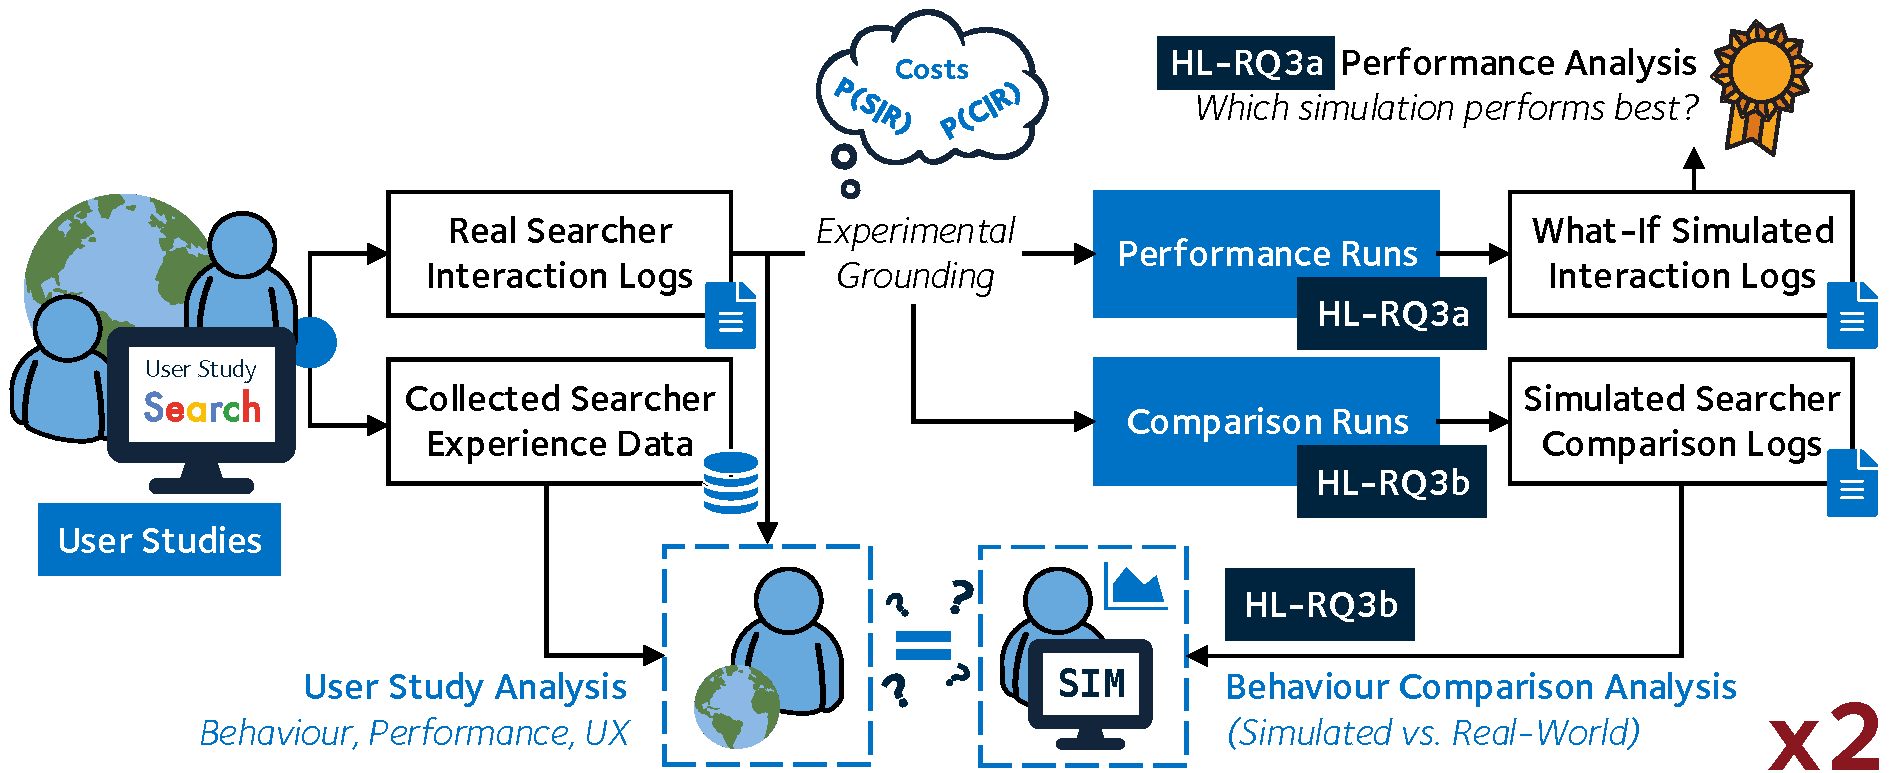
\includegraphics{figures/ch6-sim_evaluation.pdf}}
    \caption[The wider evaluation framework]{How the two sets of simulations, represented as dark blue boxes, fit within the wider experimentation framework as discussed in this chapter. The illustration also shows what components address the two high level research questions, \blueboxbold{HL-RQ3a} and \blueboxbold{HL-RQ3b}.}
    \label{fig:sim_evaluation}
\end{figure}

These simulations fit within the wider experimental framework discussed in this chapter, illustrated in Figure~\ref{fig:sim_evaluation}. Within the figure, we can see the link between the user studies and the two sets of simulations (highlighted with \darkblueboxbold{dark blue} boxes) via the act of \emph{grounding.} The illustration also provides linkage between the simulations, and the two sets of analyses that are undertaken -- the performance analysis, addressing \blueboxbold{HL-RQ3a}, and the behaviour comparison analysis that addressing \blueboxbold{HL-RQ3b}. The performance analysis is an examination of the hundreds of different possible simulation configurations, allowing us to explore how performance varies through \emph{what-if} simulations (refer to Section~\ref{sec:ir_background:user:simulation}). In all, this process is \textbf{\color{dmax_red} repeated twice}, once per user study, as shown in the illustration. We discuss the two different sets of simulations that address research questions \blueboxbold{HL-RQ3a} and \blueboxbold{HL-RQ3b} in Sections~\ref{chap:csm:method:sim:runs:performance} and~\ref{chap:csm:method:sim:runs:comparison} respectively.

One point that has not been discussed is highlighted in Figure~\ref{fig:sim_evaluation}. When executed, the simulations, employing the \simiir~framework, are saved to a series of different interaction log files. Employing the same basic structure as the real-world interaction log file illustrated in Figure~\ref{fig:log} on page~\pageref{fig:log}, the similarity between the real-world and simulated logs allowed for the same parsing infrastructure to be used with minimal changes.

\subsubsection{Performance Runs}\label{chap:csm:method:sim:runs:performance}
Named as a series of \emph{what-if} simulations above, the performance runs instantiate the different components of the~\gls{acr:csm} and \simiir~framework as previously discussed throughout Section~\ref{chap:csm:method:simulation:grounding}. Using the grounded interaction probabilities and costs, these simulations were trialled over the 50 individual topics of the~\gls{acr:trec} 2005 Robust Track~\cite{voorhees2006trec_robust}, with queries generated via the two querying strategies outlined in Section~\ref{chap:csm:method:simulation:grounding:querying}. All in all, this provided us with a wealth of simulated interaction data from which we could calculate a series of averages over the different trials experimented. As illustrated in the example figure below, we then computed the various performance measures (unless otherwise stated) over each simulated searcher configuration, taking an average over each of the 50 topics.

\begin{figure*}[h]
    \centering
    \resizebox{1\hsize}{!}{
    \vspace*{5mm}
    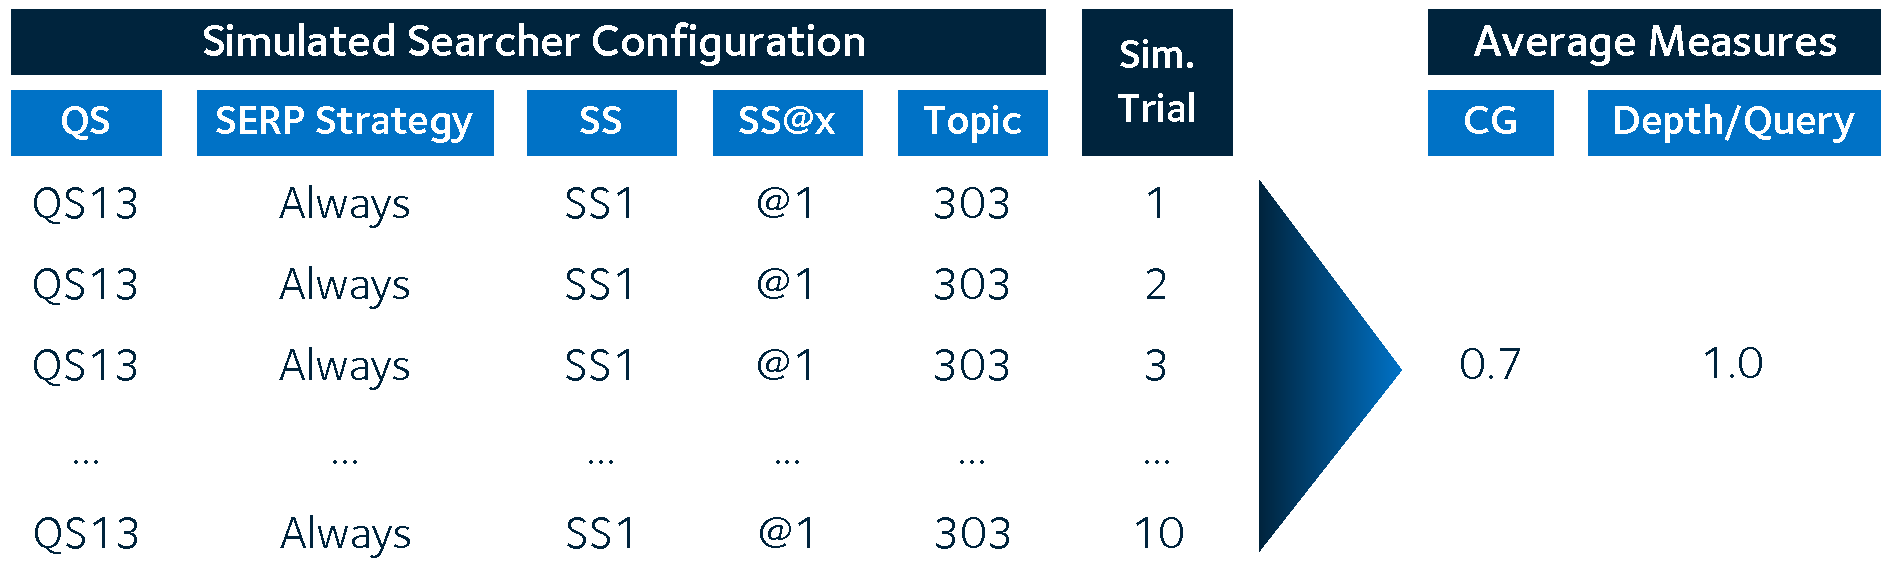
\includegraphics{figures/ch6-performance.pdf}}
    \vspace*{-6mm}
\end{figure*}

This example illustrates a single configuration of simulated searcher, using: querying strategy \blueboxbold{QS13}; the \blueboxbold{Always} (baseline)~\gls{acr:serp} examination strategy;
\stoppingstratbox{SS1-FIX}{1}; all while examining~\gls{acr:trec} topic \textnumero~303, all of which were in turn executed over ten trials. This meant that over one individual simulated search configuration, a total of $500$ simulation trials were required. Section~\ref{chap:csm:method:simulation:grounding:judgements} provides an explanation as to why these trials were required.

Given the name performance runs, we primarily examined the performance of each simulated searcher trialled. While examining the performance of queries (via the measures outlined previously in Section~\ref{sec:csm:methodology:extracting:performance}), we also examined measures illustrated in the figure above, primarily mean level of~\gls{acr:cg} attained by each simulated searcher, and the mean \blueboxbold{depth per query (D/Q)}.

\gls{acr:cg} was discussed in passing in Section~\ref{chap:csm:method:simulation:grounding:gain}. For our simulations, we consider the~\gls{acr:cg} as the amount of gain accrued over the \emph{course of a search session} -- which, by definition, can entail more than a single query. A more effective series of stopping strategies, that are better at stopping a simulated searcher examining poor quality~\glsplural{acr:serp} in any great depth, will therefore provide higher levels of~\gls{acr:cg}, but only if the queries issued offer good performance. Similarly, an effective~\gls{acr:serp} level stopping decision point implementation will stop the searcher from examining a poor~\gls{acr:serp} in the first instance, leaving more time to examine~\glsplural{acr:serp} that could potentially offer more relevant results.

The other major measure used in our performance measures was the depth per query. With this measure, performance is not measured, but rather the stopping behaviour of the simulated searchers. As shown in the illustration below, a fictional search session consists of three queries, $Q_0$, $Q_1$ and $Q_2$.

\begin{figure*}[h]
    \centering
    \resizebox{1\hsize}{!}{
    \vspace*{5mm}
    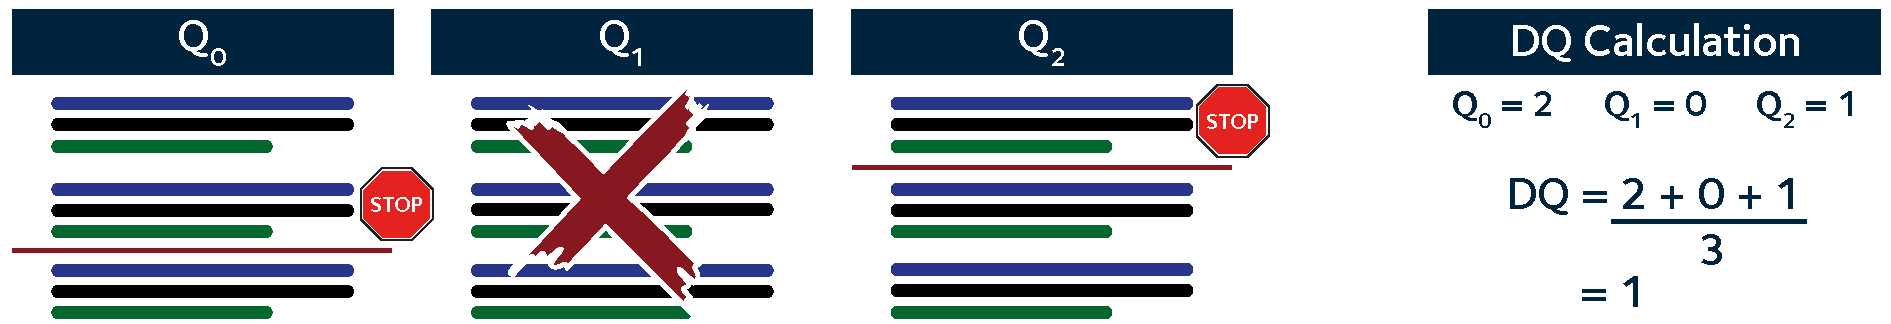
\includegraphics{figures/ch6-dq.pdf}}
    \vspace*{-6mm}
\end{figure*}

In the example, a simulated searcher examines to a depth of $2$ for $Q_0$, and a depth of $1$ for $Q_2$. The searcher does not even enter the associated~\gls{acr:serp} for $Q_1$, as the~\gls{acr:serp} level stopping decision point prevents the searcher from examining result summaries in detail. This resultant $D/Q$ for the search session is therefore $1$.

\subsubsection{Comparison Runs}\label{chap:csm:method:sim:runs:comparison}
Rather than focus upon the overall performance attained by simulated searchers under different scenarios, the second set of simulations we ran focused on comparing simulated searcher behaviours against their real-world counterparts. As such, the simulations for this set were run with minor differences in order to improve the ability for comparing the two populations of searchers -- both simulated and real-world. The first difference considered the querying component of the simulations:

\begin{itemize}
    \item{rather than considering the issuance of simulated queries via a querying strategy, we instead took the queries from the associated user study, and issued each one in turn. In effect, we \blueboxbold{replayed} all real-world queries issued.}
\end{itemize}

Following the real-world queries, we improved the realism of our simulations yet further. Queries were extracted from those issued over each individual interface and condition trialled. This also provided us with the ability to perform a direct comparison on searcher behaviour at a query level, rather than across an entire search session. However, this limited our simulations, in that:

\begin{itemize}
    \item{we considered only the \blueboxbold{four~\gls{acr:trec} topics} trialled in the user studies; the remaining 46 topics were not considered in this set of simulations.}
\end{itemize}

This was due to the fact that we only had real-world query data for the four sessions trialled in the user studies. We once again ran a simulated searcher for each different configuration, over every query issued. Ten trials were once again used, as explained in Section~\ref{chap:csm:method:simulation:grounding:judgements}.

To perform our comparisons with the real-world searchers and simulated searchers, we used the \blueboxbold{Mean Squared Error (MSE)} to compute the difference between the two. For this, our calculations were performed between the click depth of the real-world searchers over each query, and taking the simulated click depths. Simulated click depths are defined as the depth of the last document that was considered attractive enough to examine on a given simulated~\gls{acr:serp}. Considering each of simulated searcher (i.e. a combination of~\gls{acr:serp} level stopping component and snippet level stopping strategy and threshold), we could then produce a table of click depths, as provided in the example below.

\begin{figure*}[h]
    \centering
    \resizebox{1\hsize}{!}{
    \vspace*{5mm}
    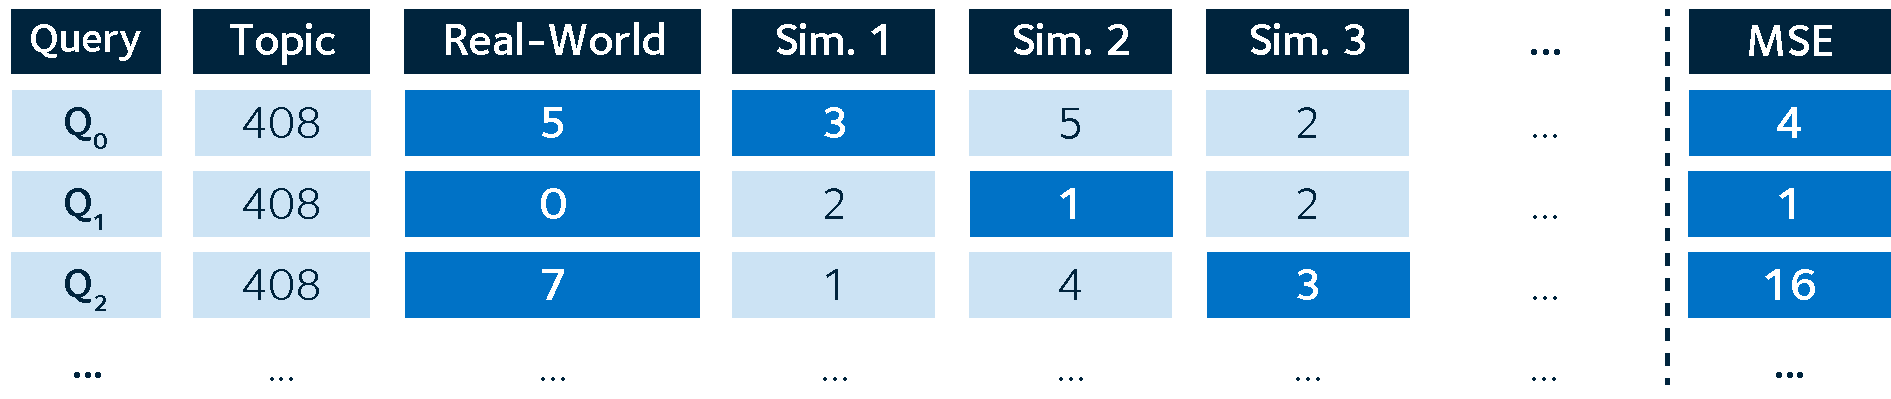
\includegraphics{figures/ch6-mse.pdf}}
    \vspace*{-6mm}
\end{figure*}

In the above, \emph{Sim. x} represents the mean value of a particular simulated searcher configuration, with the mean taken over the different simulated trials. This is the same concept as discussed previously in Section~\ref{chap:csm:method:sim:runs:performance}. For each query, the real-world click depth is shown, along with the simulated click depth from each simulated searcher trialled. The cells highlighted in light blue show what is being compared on each row -- for instance, for query $Q_0$, the real-world click depth of $5$ is compared against the \emph{Sim. 1} click depth of $3$. Considering the MSE value between the two, using the following formula:

\begin{equation*}
MSE = (\theta - \hat{\theta})^{2},
\end{equation*}

where $\theta$ denotes the real-world click depth, and $\hat{\theta}$ denotes the click depth approximation, we arrive at a MSE value of $4$. The closer the MSE value is to $0$, the better the approximation given. As such, in the above example, the compared values for $Q_1$ offer the best approximation of the actual stopping depth of the searcher. The above is just for illustration: we considered every simulated searcher, over every query. After each MSE value had been calculated, this could then be used to plot the mean depth per query across a variety of different stopping strategies. Recall, for example, that \blueboxbold{SS1-FIX} considers the stopping depth across a range of parameter values, with the parameter denoting the stopping depth. The higher this value, the greater the depth per query that will be attained. At each point, with a MSE value, we then are able to determine which stopping threshold offers the best approximation of stopping behaviour, for that particular stopping strategy.

\section{Chapter Summary}
In this chapter, we have provided an overview of the \emph{general methodology} that is used throughout the empirical work of this thesis. As we report on two separate user studies in Chapters~\ref{chap:snippets} and~\ref{chap:diversity}, this chapter provides an overview of the common approaches followed, with unique aspects discussed in the appropriate chapter.

In order to tackle the research questions posed in Section~\ref{sec:intro:rqs} on page~\pageref{sec:intro:rqs}, our general methodology was to first undertake a \blueboxbold{user study} that captured a variety of different behavioural, performance and user experience measures, as discussed in Section~\ref{sec:method:user_study}. The data derived from this user study was then used to ground a series of complex \blueboxbold{simulations of interaction}, attempting to mimic the behaviours exhibited by the real-world user study subjects. After discussing how we instantiated each of the different components of the~\gls{acr:csm} and \simiir~framework, we then concluded the chapter with a discussion on the two sets of simulation runs trialled, allowing us to address research questions \blueboxbold{HL-RQ3a} and \blueboxbold{HL-RQ3b}.

With the conclusion of this chapter, all the necessary groundwork has been laid to present the results of our user studies and simulations, which we begin in Part~\ref{part:context}.